\documentclass[../../main/main.tex]{subfiles}
\graphicspath{{./figures/}}

\dominitoc
\faketableofcontents

\makeatletter
\renewcommand{\@chapapp}{M\'ecanique -- chapitre}
\makeatother

\toggletrue{student}
% \HideSolutionstrue
% \toggletrue{corrige}
% \renewcommand{\mycol}{black}
\renewcommand{\mycol}{gray}

\begin{document}
\setcounter{chapter}{3}

\chapter{Approche \'energ\'etique du mouvement}

\vspace*{\fill}

\begin{prgm}
	\begin{tcb}*(ror)"know"{Savoirs}
		\begin{itemize}
			\item Puissance et travail d'une force dans un référentiel.
			\item Théorèmes de l'énergie cinétique et de la puissance cinétique dans
			      un référentiel galiléen.
			\item Utiliser le théorème approprié en fonction du contexte.
			\item Énergie potentielle. Lien entre un champ de force conservative et
			      l'énergie potentielle. Gradient.
			\item Énergie mécanique. Théorème de l'énergie mécanique. Mouvement
			      conservatif.
			\item Positions d'équilibre. Stabilité.
		\end{itemize}
	\end{tcb}
	\begin{tcb}*(ror)"how"{Savoir-faire}
		\begin{itemize}
			\item Établir et citer les expressions de l'énergie potentielle de
			      pesanteur (champ uniforme), de l'énergie potentielle
			      gravitationnelle (champ créé par un astre ponctuel), de l'énergie
			      potentielle élastique.

			\item Déterminer l'expression d'une force à partir de l'énergie
			      potentielle, l'expression du gradient étant fournie.

			\item Déduire qualitativement, en un point du graphe d'une fonction
			      énergie potentielle, le sens et l'intensité de la force associée.

			\item Distinguer force conservative et force non conservative, reconnaître
			      les cas de conservation de l'énergie mécanique.

			\item Déduire d'un graphe d'énergie potentielle le comportement
			      qualitatif~: trajectoire bornée ou non, mouvement périodique,
			      positions de vitesse nulle.

			\item Déduire d'un graphe d'énergie potentielle l'existence de positions
			      d'équilibre. Analyser qualitativement la nature, stable ou instable,
			      de ces positions.

			\item Établir l'équation différentielle du mouvement au voisinage d'une
			      position d'équilibre.
		\end{itemize}
	\end{tcb}
\end{prgm}

\vspace*{\fill}

\newpage

\vspace*{\fill}
\minitoc
\vspace*{\fill}

\newpage

% \vspace*{\fill}
% \begin{boxes}
{
	\footnotesize
	\begin{tcb}(defi)<lftt>{Liste des définitions}
		\tcblistof[\paragraph*]{defi}{\hspace*{3pt}}
	\end{tcb}
	\vspace{-10pt}
	% \begin{tcb}(rapp)<lftt>{Liste des rappels}
	% 	\tcblistof[\paragraph*]{rapp}{\hspace*{6pt}}
	% \end{tcb}
	\begin{tcb}(prop)<lftt>{Liste des propriétés}
		\tcblistof[\paragraph*]{prop}{\hspace*{3pt}}
	\end{tcb}
	\vspace{-10pt}
	% \begin{tcb}(coro)<lftt>{Liste des corollaires}
	% 	\tcblistof[\paragraph*]{coro}{\hspace*{3pt}}
	% \end{tcb}
	\begin{tcb}(demo)<lftt>{Liste des démonstrations}
		\tcblistof[\paragraph*]{demo}{\hspace*{3pt}}
	\end{tcb}
	\vspace{-10pt}
	% \begin{tcb}(inte)<lftt>{Liste des interprétations}
	% 	\tcblistof[\paragraph*]{inte}{\hspace*{3pt}}
	% \end{tcb}
	\begin{tcb}(tool)<lftt>{Liste des outils}
		\tcblistof[\paragraph*]{tool}{\hspace*{3pt}}
	\end{tcb}
	\vspace{-10pt}
	% \begin{tcb}(nota)<lftt>{Liste des notations}
	% 	\tcblistof[\paragraph*]{nota}{\hspace*{3pt}}
	% \end{tcb}
	\begin{tcb}(appl)<lftt>{Liste des applications}
		\tcblistof[\paragraph*]{appl}{\hspace*{3pt}}
	\end{tcb}
	\vspace{-10pt}
	% \begin{tcb}(rema)<lftt>{Liste des remarques}
	% 	\tcblistof[\paragraph*]{rema}{\hspace*{3pt}}
	% \end{tcb}
	% \begin{tcb}(exem)<lftt>{Liste des exemples}
	% 	\tcblistof[\paragraph*]{exem}{\hspace*{3pt}}
	% \end{tcb}
	\begin{tcb}(ror)<lftt>{Liste des points importants}
		\tcblistof[\paragraph*]{ror}{\hspace*{3pt}}
	\end{tcb}
	\vspace{-10pt}
	\begin{tcb}(impo)<lftt>{Liste des erreurs communes}
		\tcblistof[\paragraph*]{impo}{\hspace*{3pt}}
	\end{tcb}
	% \end{boxes}
	% \vspace*{\fill}
}
\newpage

\section{Notions énergétiques}
\subsection{Énergie}
L'énergie est un concept physique très puissant et présent dans tout les
domaines de la physique mais qu'il est difficile de définir simplement. En voici
une première définition qualitative~:
\begin{tcb*}[sidebyside, righthand ratio=.3](defi){Énergie}
	L'énergie d'un système est sa capacité à agir sur lui-même ou d'autres
	systèmes.
	\tcblower
	Unité~: le \textbf{Joule} (J)
\end{tcb*}

Ainsi, le mouvement d'un corps, les échanges de chaleur, les courants
électriques et tous les phénomènes physiques résultent d'échanges d'énergie.
Elle respecte une propriété principale, fondamentale de l'approche du monde qui
nous entoure~:

\begin{tcb*}(prop){Conservation de l'énergie}
	\bfseries
	L'énergie est une grandeur conservative. Elle ne peut être créée ou
	détruite. Elle ne peut que changer de forme et/ou passer d'un système à un
	autre.
\end{tcb*}

Ces notions serons retravaillées en thermodynamique.

\vspace{-10pt}
\subsection{Puissance}

Une énergie totale peut varier différemment selon les conditions du système, et
notamment varier plus ou moins vite. Cette variation est une information
caractéristique de l'évolution d'un système~: une voiture qui freine pour
diminuer son énergie cinétique peut le faire lentement ou rapidement et
donnerons des ressentis physiques très différents. On définit pour ça la
puissance d'un système~:

\begin{tcb*}[sidebyside](defi){Puissance en terme d'énergie}
	La \textbf{puissance} $\Pc$ d'un système traduit la \textbf{variation
		temporelle} de son énergie $\Ec$, et on a
	\[\boxed{\Pc = \dv{\Ec}{t}}\]
	\tcblower
	L'unité d'une puissance est donc homogène à des $\si{J.s^{-1}}$, et se compte
	couramment en \textbf{Watts} (W). On a
	\[\boxed{\SI{1}{W} = \SI{1}{J.s^{-1}}}\]
\end{tcb*}

\begin{tcb*}(impo){Puissance d'une force}
	Pratique pour retrouver son unité, cette expression est cependant peu
	utilisée~; en effet, lors de l'étude mécanique d'un corps, on connaît moins
	facilement son énergie que sa vitesse ou les forces qui s'y appliquent. On
	verra la Définition~\ref{defi:pforce} qui est plus utile.
\end{tcb*}

\vspace{-10pt}
\section{Énergie cinétique et travail d'une force constante}
\vspace{-5pt}
\subsection{Énergie cinétique}
\vspace{-10pt}
\begin{tcb*}[sidebyside](defi){Énergie cinétique}
	L'énergie cinétique d'un point M de masse $m$ et de vitesse $v\Rg(\Mr)$ est~:
	\psw{
		\[\boxed{\Ec_{c}\Rg(\Mr) = \frac{1}{2}mv\Rg(\Mr)^2}\]
	}
	\vspace{-15pt}
	\tcblower
	L'unité d'une énergie est en \fbox{\textbf{joules}} (J), et dépend du
	référentiel.
\end{tcb*}

\subsection{Travail d'une force}

\noindent
\textbf{À quelle condition une force appliquée à un objet fait-elle varier son
	énergie cinétique~?}
\begin{itemize}
	\item Quand un objet est jeté vers le haut, le poids le ralentit, donc fait
	      diminuer son énergie cinétique.
	\item Quand un objet tombe, le poids l'accélère et fait donc augmenter son
	      énergie cinétique.
	\item Lorsqu'un objet est posé sur un support, la réaction normale ne fait
	      pas varier son énergie cinétique.
	\item Lorsqu'un objet freine sur un support horizontal, la réaction normale
	      ne cause pas la variation de son énergie cinétique (c'est la réaction
	      tangentielle qui le freine).
\end{itemize}
\begin{tcb*}[bld, cnt](inte){Travail d'une force}
	Le travail est une grandeur physique construite pour rendre compte de
	l'effet d'une force sur son énergie cinétique.
\end{tcb*}

\begin{itemize}
	\item En l'absence de déplacement, le travail doit être nul.
	\item Si la force est perpendiculaire au déplacement, le travail doit être
	      nul.
	\item Si la force est dans le sens du déplacement, le travail doit être
	      positif et maximal.
	\item Si la force est dans le sens opposé au déplacement, le travail doit
	      être négatif (et minimale).
\end{itemize}

\begin{tcb*}[sidebyside, sidebyside align=top](defi)
	{Travail d'une force constante}
	Le travail $W_{\ABr}$ d'une force \textbf{constante} $\Ff$ sur un chemin $\ABf$ est
	\psw{
		\[\boxed{W_{\ABr}(\Ff) = \Ff\cdot\ABf}\]
	}
	où «~$\cdot$~» désigne le produit scalaire entre deux vecteurs.
	\tcblower
	\tcbsubtitle{\fatbox{Unité}}
	\psw{
		Un \textbf{travail} est homogène à une \textbf{énergie}, donc s'exprime en
		\fbox{\textbf{joules}}.
	}
\end{tcb*}

\begin{tcb*}(ror)<lftt>'l'{Vocabulaire et conséquence du travail}
	\begin{itemize}
		\item \psw{
			      Si $W_{\ABr} > 0$, on dit que le travail est \textbf{moteur}~; si
			      $W_{\ABr} < 0$ il est \textbf{résistant}.
		      }
		\item \psw{
			      $W_{\ABr} = 0 \Ra$ soit $\Ff = \of$, soit $\ABf = \of$, soit
			      $\ABf\perp\Ff$.
		      }
	\end{itemize}
\end{tcb*}

\subsection{Exemples de travaux}

\begin{tcb*}[breakable](tool){Calculer un travail}
	On peut calculer un travail avec deux formes mathématiques équivalentes~:
	\begin{itemize}
		\item En utilisant une base de projection, \textit{par exemple} cartésienne,
		      on décompose la force et le déplacement~:
		      \psw{
			      \[
				      \Ff = F_x\ux + F_y\uy + F_z\uy
				      = \mqty(F_x\\F_y\\F_z)
				      \qet
				      \ABf = x\ux + y\uy + z\uz
				      = \mqty(x\\y\\z)
			      \]
		      }
		      On a alors
		      \psw{
			      \[
				      \boxed{\Ff\cdot\ABf = xF_x + yF_x + zF_z}
				      =
				      \mqty{\\+\\+}
				      \mqty(F_x\\F_y\\F_z)
				      \mqty{\times\\\times\\\times}
				      \mqty(x\\y\\z)\]
		      }
		\item En utilisant une autre définition du produit scalaire~:
		      \psw{
			      \[\boxed{\Ff\cdot\ABf = \norm{\Ff}\times\norm{\ABf}\cos\a}\]
		      }
		      avec $\a$ l'angle entre les vecteurs.
	\end{itemize}
\end{tcb*}

\begin{tcb*}(appl)<lftt>'l'{Travail des frottements solides}
	On a vu en TD qu'un objet, de vitesse initiale $v_0\ux$, soumis à une force
	de frottements solides sur un support horizontal subissait, lors de son
	mouvement avec glissement,
	\psw{
		\[\Tf = -fmg\ux\]
	}
	et parcourait pendant la phase de freinage la distance
	\psw{
	\[D = \frac{v_0{}^2}{2fg}\]
	}
	\begin{enumerate}[label=\sqenumi]
		\item Calculer le travail de la force de frottements sur cette distance.
		      Est-il moteur ou résistant~?
		\item Que vaut $\Ec_{c,0}$ l'énergie cinétique initale~? $\Ec_{c,\infty}$
		      sont énergie cinétique finale~? Que peut-on en conclure~?
	\end{enumerate}
	\tcblower
	\begin{enumerate}[label=\sqenumi]
		\mitem \psw{
			\begin{align*}
				W_{\ABr}(\Ff)         & = \Ff\cdot\ABf
				\\\Lra
				W_{\ABr}(\Ff)         & = \norm{\Ff}\times\norm{\ABf}\times\cos(\pi)
				\\\Lra
				W_{\ABr}(\Ff)         & = fmg\times\frac{v_0{}^2}{2fg}\times(-1)
				\\\Lra
				\Aboxed{W_{\ABr}(\Ff) & = - \frac{1}{2}mv_0{}^2}
			\end{align*}
			Le travail étant négatif, on dit qu'il est (et que la force est)
			\textbf{résistant}(e).}
		\mitem \psw{
			\begin{gather*}
				\Ec_{c,0} = \frac{1}{2}mv_0{}^{2}
				\\
				\Ec_{c,\infty} = 0
				\\\Ra
				\boxed{W_{\ABr} = \Delta_{\ABr}{\Ec_{c}}}
			\end{gather*}
			On observe que l'énergie initiale du système, son
			énergie cinétique, a été dissipée par la force de frottements et est
			quantifiée par le travail de cette force sur le chemin suivi.
		}
	\end{enumerate}
\end{tcb*}

\begin{tcb*}[breakable](appl)<lftt>'l'{Travail du poids}
	Calculer le travail du poids lors d'un déplacement avec changement
	d'altitude.
	\tcblower
	\begin{minipage}{0.25\linewidth}
		\begin{center}
			\sswitch{
				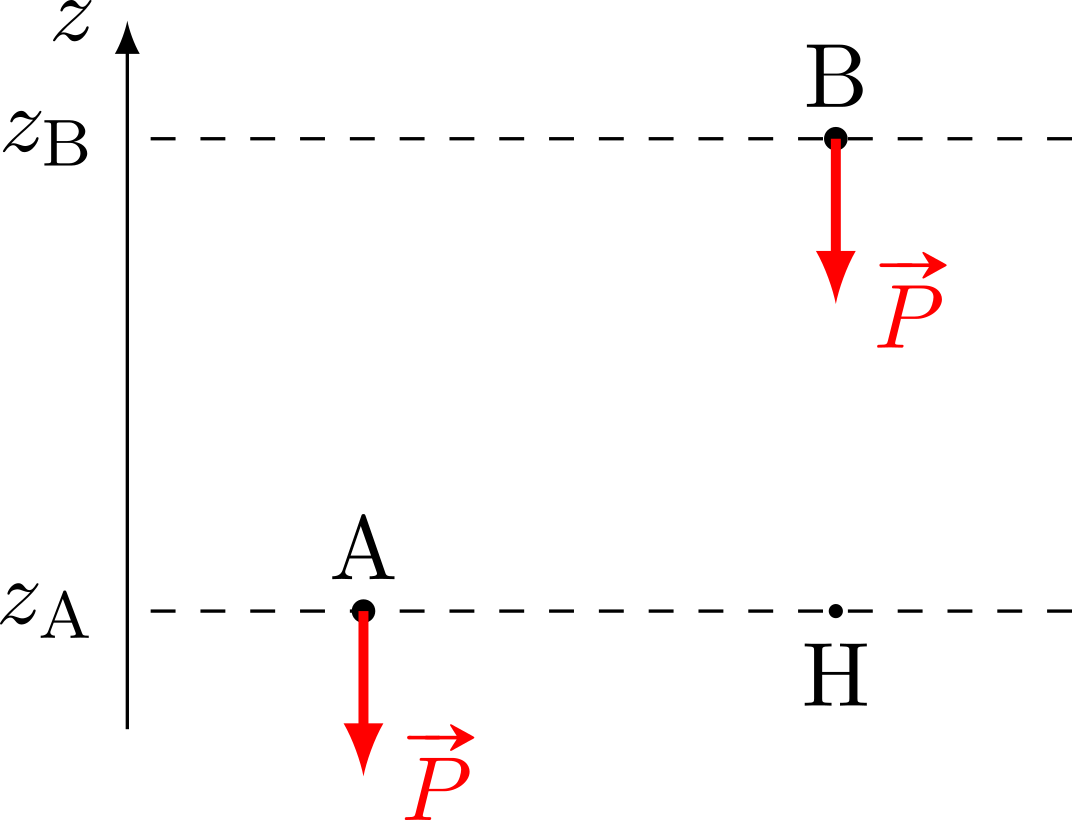
\includegraphics[width=.8\linewidth, draft=true]{w_p}
			}{
				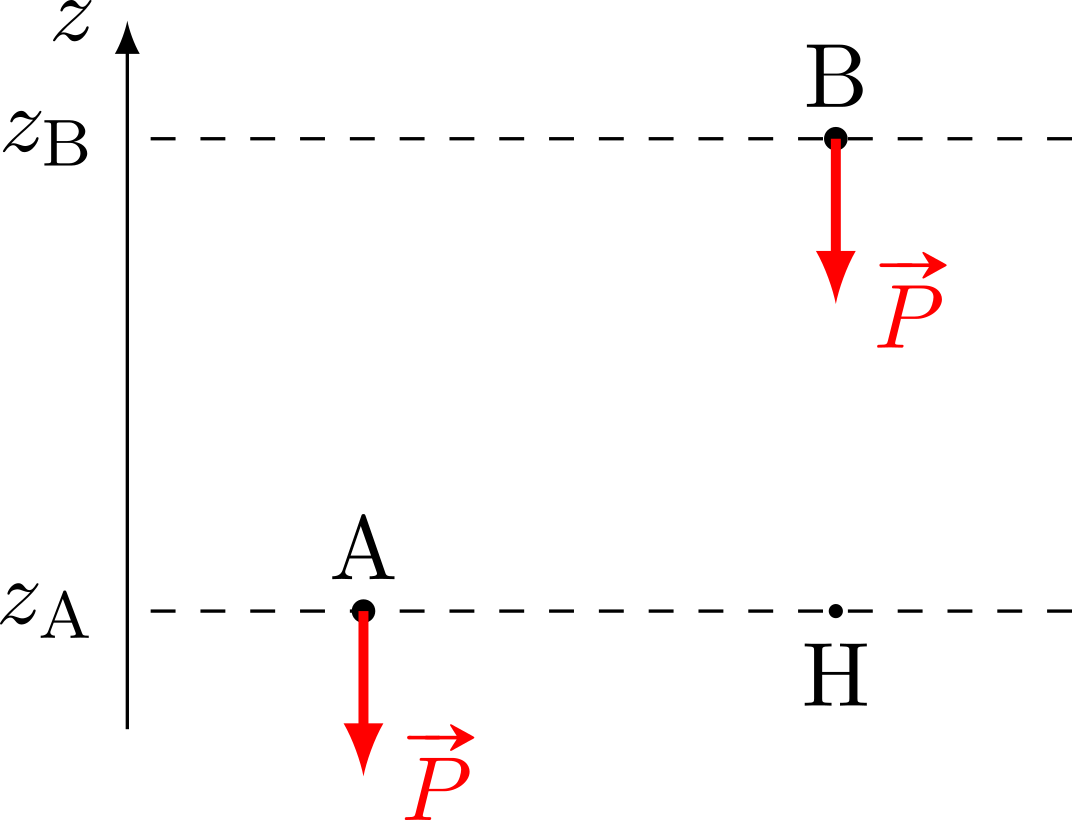
\includegraphics[width=.8\linewidth]{w_p}
			}
			\vspace{-10pt}
			\captionsetup{justification=centering}
			\captionof{figure}{Schéma}
		\end{center}
	\end{minipage}
	\hfill
	\begin{minipage}{.75\linewidth}
		\psw{
			\[W_{\ABr}(\Pf) = \Pf\cdot\ABf\]
			En projection cartésienne~:
			\begin{gather*}
				\Pf = -mg\uz
				\qet
				\ABf = (x_\Br-x_\Ar)\ux + (y_\Br - y_\Ar)uy + (z_\Br - z_\Ar)\uz
				\\
				W_{\ABr}(\Pf) = -mg(z_\Br - z_\Ar)
			\end{gather*}
		}
	\end{minipage}
	\vspace*{-15pt}
\end{tcb*}

\begin{tcb*}(prop){Travail du poids}
	Le travail du poids entre un point A et un point B est~:
	\psw{
		\[\boxed{W_\ABr(\Pf) = mg(z_\Ar - z_\Br)}\]
	}
	\vspace{-15pt}
\end{tcb*}

\begin{tcb*}(appl)<lftt>'l'{Travail des frottements fluides}
	On considère une voiture allant d'un point A à un point B, éloignés de
	\SI{100}{km}, avec une vitesse constante. La force de frottement exercée par
	l'air est
	\[\Ff = -\frac{1}{2}\rho Sc_xv\vf\]
	Déterminer son travail, et faire l'application
	numérique pour $v = \SI{50}{km.h^{-1}}$ puis \SI{80}{km.h^{-1}}. On donne $S
		= \SI{3.07}{m^2}$, $c_x = \num{0.33}$, $\rho = \SI{1.3}{kg.m^{-3}}$.
	\tcblower
	\begin{minipage}{0.45\linewidth}
		\begin{center}
			\sswitch{
				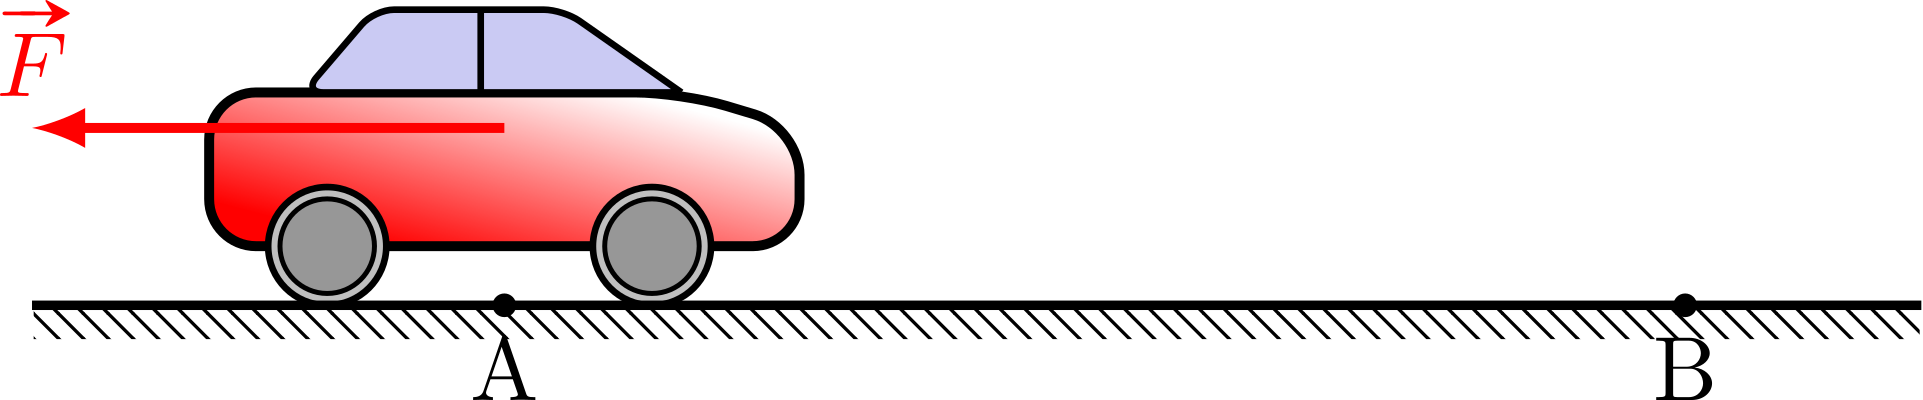
\includegraphics[width=\linewidth, draft=true]{voiture}
			}{
				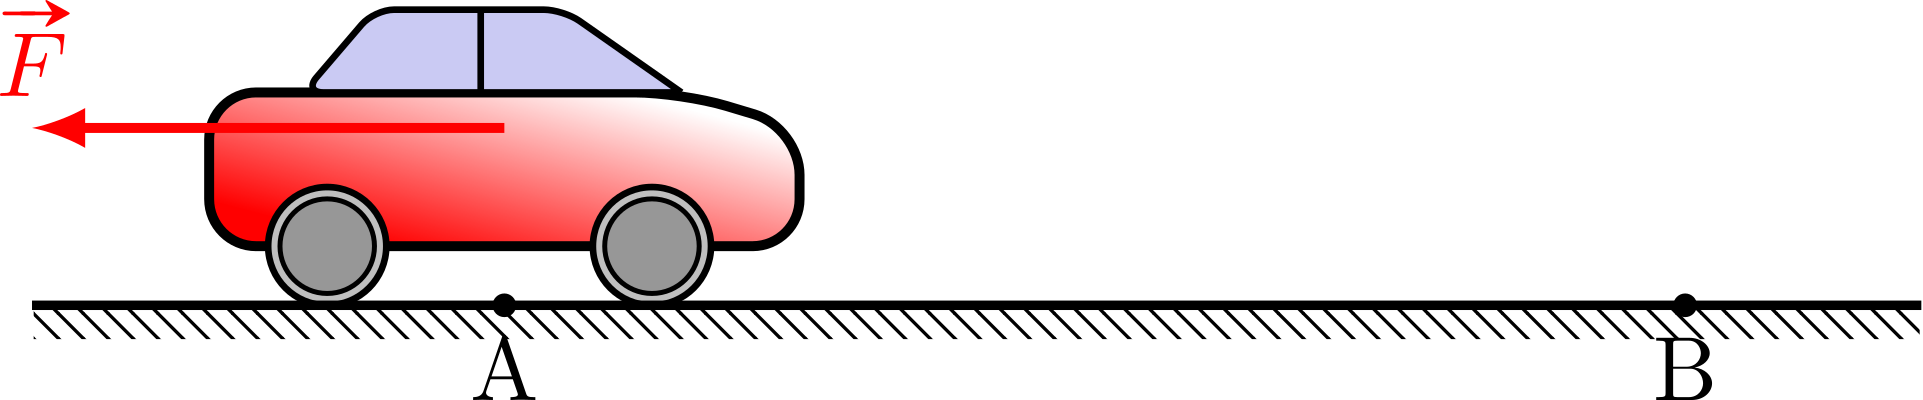
\includegraphics[width=\linewidth]{voiture}
			}
			\vspace{-15pt}
			\captionof{figure}{Schéma}
		\end{center}
	\end{minipage}
	\hfill
	\begin{minipage}{0.45\linewidth}
		\psw{
			\[W_{\ABr}(\Ff) = \Ff\cdot\ABf = -F\times\ABr\]
			Le travail est négatif, la force est résistante.
			\begin{itemize}
				\item $v = \SI{50}{km.h^{-1}} \Ra W_{\ABr}(\Ff) = \SI{-1.27e7}{J}$,
				      soit $\approx \SI{0.4}{L}$ d'essence~;
				\item $v = \SI{80}{km.h^{-1}} \Ra W_{\ABr}(\Ff) = \SI{-3.25e7}{J}$,
				      soit $\approx \SI{1}{L}$ d'essence.
			\end{itemize}
		}
	\end{minipage}
\end{tcb*}

Ainsi, dans certains cas le travail ne dépend pas que du point de départ et
d'arrivée, mais peut dépendre de la \textbf{façon} d'y aller (vitesse, chemin
suivi…). En realité,
\begin{tcb*}[cnt, bld](ror){Travail et chemin}
	De façon générale, le travail dépend du chemin suivi.
\end{tcb*}

\section{Puissance et travail élémentaire}
\subsection{Travail élémentaire}
\begin{tcb*}(defi){Travail élémentaire}
	Le travail élémentaire $\de W$ d'une force $\Ff$ sur un déplacement
	infinitésimal $\dd\OM$ est~:
	\psw{
		\[\boxed{\de W = \Ff\cdot\dd\OM}\]
	}
	\vspace*{-15pt}
\end{tcb*}
\vspace*{-15pt}
\begin{tcb*}(impo){Notations $\de$ vs. $\dd$}
	$\de \Ra$ grandeur totale dépend \textit{a priori} du chemin et de la vitesse.
	$\dd{} \Ra$ grandeur dépend uniquement du point de départ et du point
	d'arrivée~; or $W$ défini sur une \textbf{distance}, pas
	\cancel{\bcancel{\textbf{en un point}}}~:
	\begin{gather*}
		\psw{\int_\Ar^\Br \dd\Ec_c = \Ec_c(\Br) - \Ec_c(\Ar)}
		\qet
		\psw{\int_\Ar^\Br \dd\OM = \vv{\rm OB} - \vv{\rm OA} = \ABf}
		\\
		\beforetext{mais il est absurde d'écrire}
		\psw{
			\cancel{\bcancel{
					\int_{\Ar}^{\Br} \de W = W(\Br) - W(\Ar)
				}}
		}
	\end{gather*}
	\vspace{-15pt}
\end{tcb*}

% \begin{tcb*}(inte){Travail élémentaire et énergie cinétique}
% 	La variation d'énergie cinétique due à une force $\Ff$ pendant un temps
% 	infinitésimal $\dt$ est celui des travaux élémentaires
% 	\[\dd\Ec_c = \sum \Ff\cdot\dd{\OM}\]
% \end{tcb*}

\subsection{Puissance}
Si la puissance est en effet la dérivée d'une énergie par rapport au temps, on
peut l'exprimer comme étant la rapidité avec laquelle un travail (homogène à une
énergie) peut être effectué.
\begin{tcb*}[sidebyside, label=defi:pforce, righthand ratio=.25, sidebyside
		align=top](defi) {Puissances d'une force}
	\begin{isd}[sidebyside align=top]
		\tcbsubtitle{\fatbox{\textbf{Moyenne}}}
		\psw{
			\[\Pc_m = \frac{W_{\ABr}(\Ff)}{\Dt}\]
		}
		\tcblower
		\tcbsubtitle{\fatbox{\textbf{Instantanée}}}
		\vspace{-15pt}
		\psw{
			\begin{gather*}
				\Pc\Rg(\Ff) = \frac{\delta W(\Ff)}{\dd{t}}
				\\\Lra
				\boxed{\Pc\Rg(\Ff) = \Ff\cdot\vf\Rg}
			\end{gather*}
		}
		\vspace{-15pt}
	\end{isd}
	\tcblower
	\tcbsubtitle{\fatbox{Unité}}
	Les \textbf{watts} (W).
	\smallbreak
	Elle dépend du référentiel.
\end{tcb*}

\begin{tcb*}[breakable](appl)<lftt>'l'{Puissance du poids en pente}
	Exprimer la puissance du poids lors d'une descente à vélo d'une pente
	d'angle $\a$.
	\tcblower
	\begin{minipage}{0.35\linewidth}
		\begin{center}
			\sswitch{
				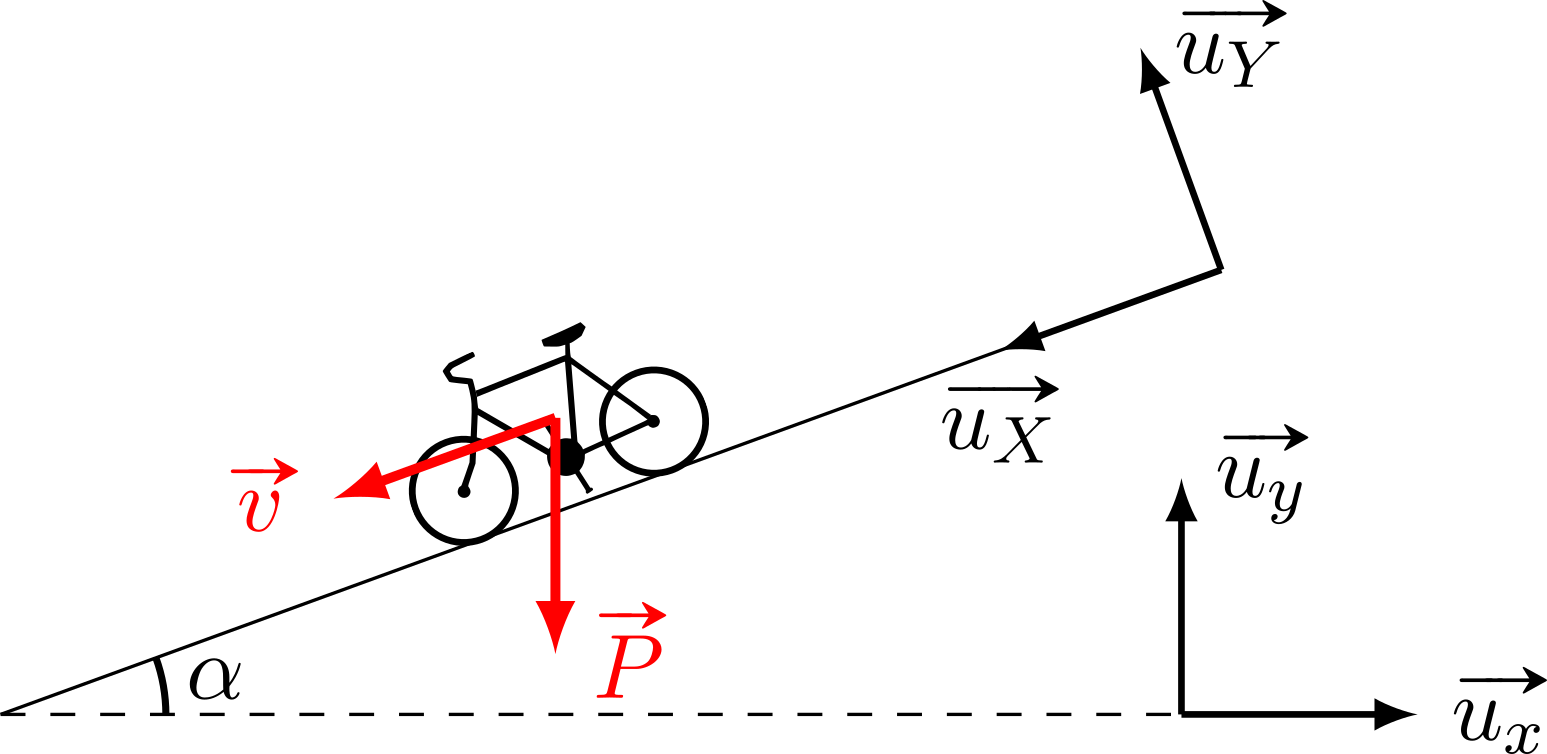
\includegraphics[width=\linewidth, draft=true]{velo}
			}{
				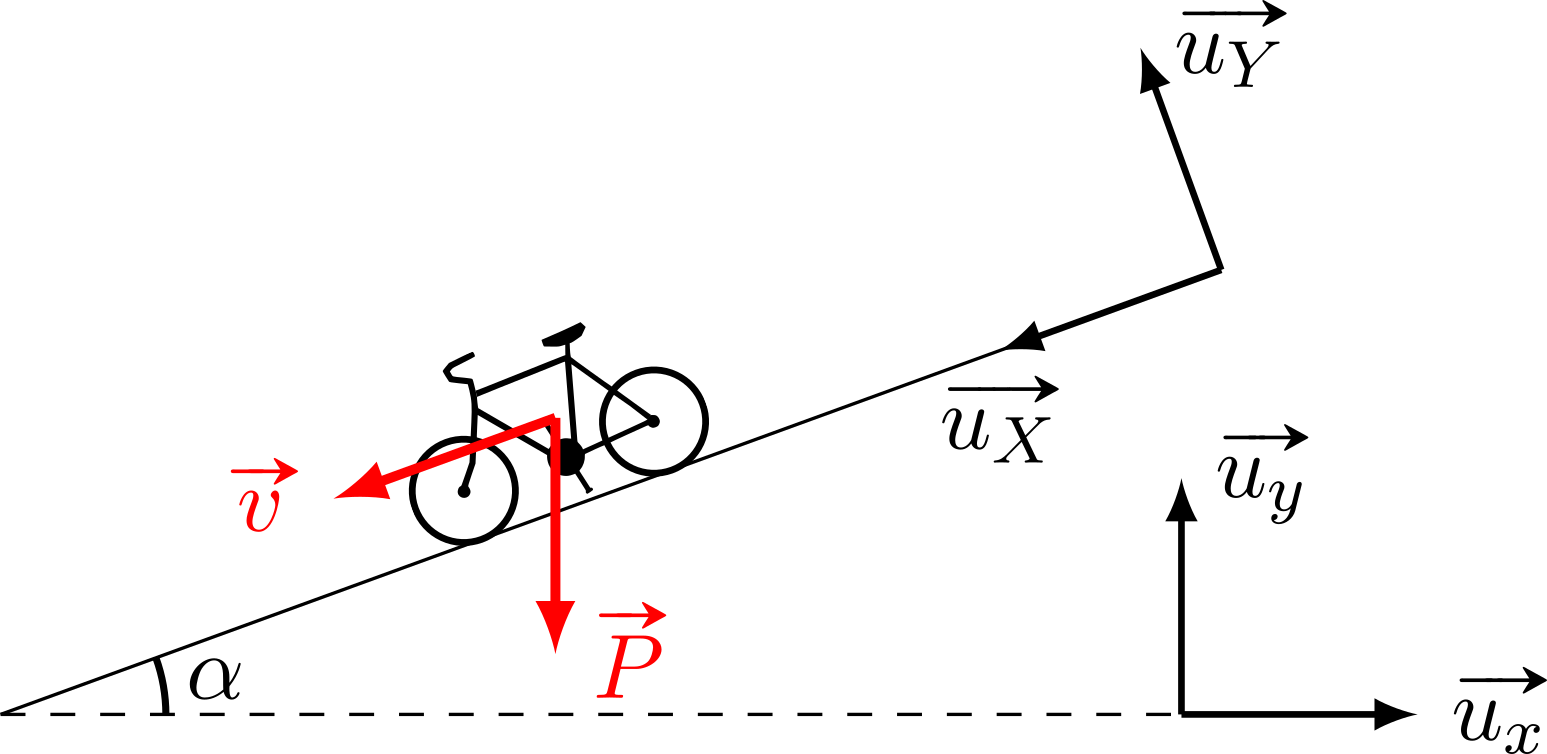
\includegraphics[width=\linewidth]{velo}
			}
			\vspace{-15pt}
			\captionof{figure}{Schéma}
		\end{center}
	\end{minipage}
	\hfill
	\begin{minipage}{0.60\linewidth}
		Dans la base $(\vv{u_X},\vv{u_Y})$~:
		\psw{
			\begin{gather*}
				\Pf = m\gf = mg(-\cos\a\vv{u_Y} + \sin\a\vv{u_X})
				\\\text{et}\quad
				\vf = v\vv{u_X}
			\end{gather*}
		}
		Ainsi, dans le référentiel de la route~:
	\end{minipage}\bigbreak
	\psw{
		\[
			\boxed{
				\Pc(\Pf) = \Pf\cdot\vf = mgv\sin\a
			}
			\quad >0 \quad \Ra \quad \text{poids moteur}
		\]
	}
	\psw{
		Dans le cas de la montée, on inverse le sens de $\vf$, et le poids
		devient résistant.
	}
\end{tcb*}

\begin{tcb*}(impl){Puissance d'une force perpendiculaire}
	Par conséquence du produit scalaire, \textbf{toute force perpendiculaire au
		mouvement a un travail nul et une puissance nulle}.
\end{tcb*}

\vspace{-15pt}
\subsection{Théorème de la puissance cinétique}

\begin{tcb*}(demo){Théorème de la puisance cinétique}
	Deux méthodes possibles pour la démonstration~:
	\smallbreak
	\begin{isd}[sidebyside align=top]
		\tcbsubtitle{\fatbox{\textbf{Bilan de puissance}}}
		\vspace*{-15pt}
		\psw{
			\begin{align*}
				m\af                          & = \sum_i \Ff_i
				\\\Lra
				m \dv{\vf}{t}\cdot\vf         & = \sum_i \Ff_i\cdot\vf
				\\\Lra
				\dv{t}(\frac{1}{2}mv^2)       & = \sum_i \Pc(\Ff_i)
				\\\Lra
				\Aboxed{\dv{\Ec_c\Rg(\Mr)}{t} & = \sum_i \Pc\Rg(\Ff_i)}
				\qed
			\end{align*}
		}
		\vspace{-15pt}
		\tcblower
		\tcbsubtitle{\fatbox{\textbf{Définition de $\Ec_c$}}}
		\vspace*{-15pt}
		\psw{
			\begin{align*}
				\dv{\Ec_c}{t} & = \dv{t}(\frac{1}{2}m\vf\cdot\vf)
				\\
				              & = \frac{1}{2}m \left( \vf\cdot \dv{\vf}{t} + \dv{\vf}{t}
				\cdot \vf\right)
				\\
				              & = m\dv{\vf}{t}\cdot\vf
				\\\Lra
				\dv{\Ec_c}{t} & = \left( \sum_i \Ff_i \right)\cdot\vf
				\qed
			\end{align*}
		}
		\vspace{-15pt}
	\end{isd}
\end{tcb*}

% \begin{tcb*}(demo)<lftt>'l'{Démonstration}
%     Différentes démonstrations sont possibles, soit en faisant un bilan de
%     puissance (c'est-à-dire PFD$\times\vf$), soit en partant de la définition de
%     l'énergie cinétique~:
%     \begin{rsidedemo}
%         \vspace{-10pt}
%         \begin{align*}
%             m\af &= \sum_i \Ff_i
%             \\\Lra
%             m \dv{v}{t}\cdot\vf &= \sum_i \Ff_i\cdot\vf
%             \\\Lra
%             \dv{t}(\frac{1}{2}mv^2) &= \sum_i \Pc(\Ff_i)
%             \\\Lra
%             \Aboxed{\dv{\Ec_c\Rg(\Mr)}{t} &= \sum_i \Pc\Rg(\Ff_i)}
%         \end{align*}
%         \tcblower
%         \vspace{-10pt}
%         \begin{align*}
%             \dv{\Ec_c}{t} &= \dv{t}(\frac{1}{2}m\vf\cdot\vf)
%             \\
%                           &= \frac{1}{2}m \left( \vf\cdot \dv{\vf}{t} + \dv{\vf}{t}
%                           \cdot \vf\right)
%             \\
%                           &= m\dv{\vf}{t}\cdot\vf
%             \\\Lra
%             \dv{\Ec_c}{t} &= \left( \sum_i \Ff_i \right)\cdot\vf
%         \end{align*}
%     \end{rsidedemo}
% \end{tcb*}

\begin{tcb*}(theo){de la puissance cinétique}
	Dans un référentiel galiléen $\Rc$, la variation instantanée de l'énergie
	cinétique d'un point matériel M est égale à la somme des puissances de
	forces qui s'exercent sur ce point~:
	\psw{
		\[\boxed{\dv{\Ec_c\Rg(\Mr)}{t} = \sum_i \Pc\Rg(\Ff_i)}\]
	}
	\vspace{-15pt}
\end{tcb*}

\begin{tcb*}(appl)<lftt>'l'{Conséquence énergétique des frottements}
	Justifier que les frottements conduisent à une baisse de l'énergie
	cinétique.
	\tcblower
	\vspace{-15pt}
	\begin{gather*}
		\psw{\Ff_{f}\cdot\vf < 0}
		\quad \Ra \quad
		\psw{\Pc\Rg(\Ff_f) < 0}
		\quad \Ra \quad
		\psw{\boxed{\dv{\Ec_c}{t} < 0}}
	\end{gather*}
	\vspace*{-25pt}
\end{tcb*}
\vspace{-15pt}
\begin{tcb*}(appl)<lftt>'l'{Pendule \textit{via} TPC}
	Établir l'équation différentielle du pendule.
	\tcblower
	\begin{minipage}{0.25\linewidth}
		\begin{center}
			\sswitch{
				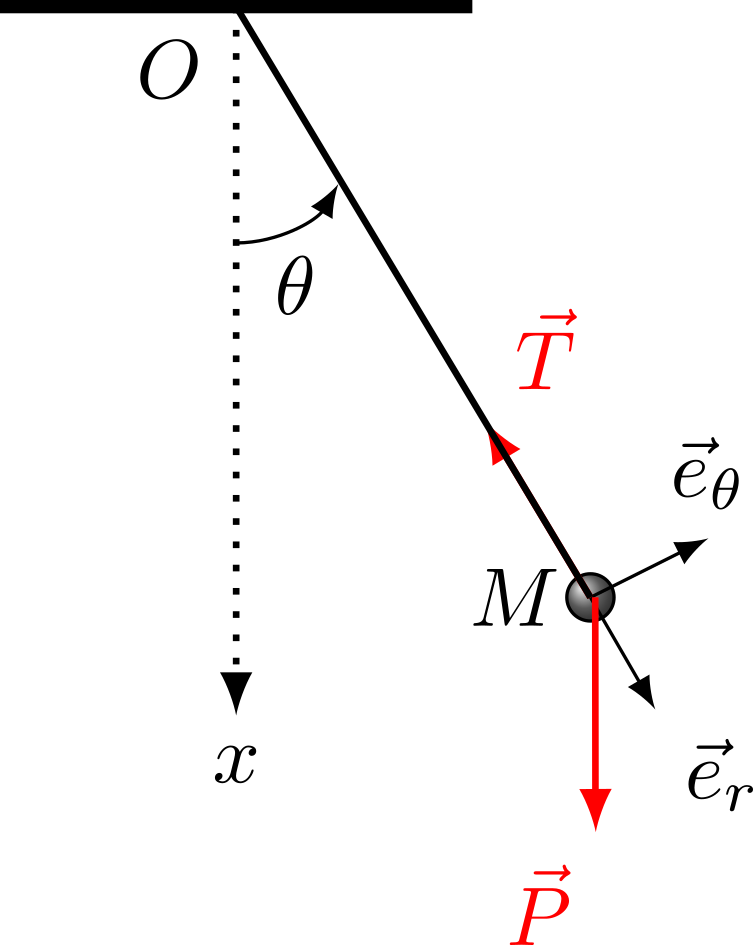
\includegraphics[width=.8\linewidth, draft=true]{pendule_plain}
			}{
				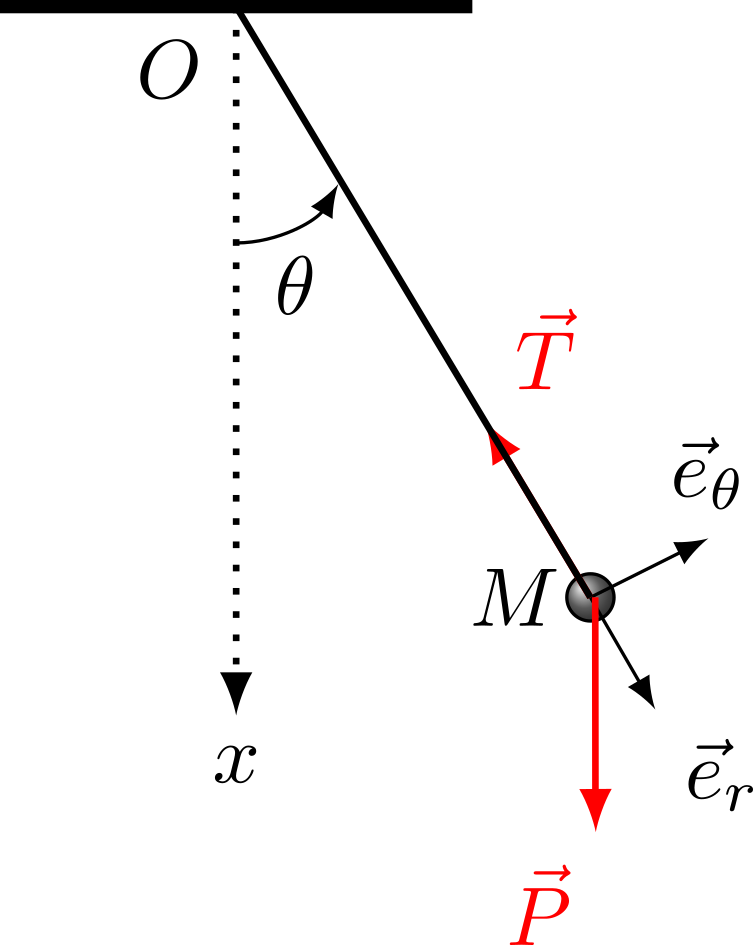
\includegraphics[width=.8\linewidth]{pendule_plain}
			}
			\vspace{-15pt}
			\captionof{figure}{Pendule}
		\end{center}
	\end{minipage}
	\hfill
	\begin{minipage}{0.70\linewidth}
		Le mouvement étant circulaire, $\vf = \ell\tp\ut$ et on a
		\begin{gather*}
			\psw{\Ec_c = \frac{1}{2}m\ell^2\tp^2}
			\Ra
			\psw{\dv{\Ec_c}{t} = m\ell^2\tp\tpp}
		\end{gather*}
		De plus, $\vf\perp\Tf$ et l'angle entre $\vf$ et $\Pf$ est $\pi/2+\tt$~:
		\begin{gather*}
			\psw{\Tf\cdot\vf = 0}
			\qet
			\psw{
				\Pf\cdot\vf = mg\times\ell\tp\times\cos(\frac{\pi}{2}+\tt) =
				-mg\ell\tp\sin\tt
			}
			\\
			\beforetext{TPC $\Ra$}
			\psw{
				\cancel{m\ell^2\tp}\tpp =
				0 - \frac{
					\cancel{m}g\dcancel{\ell}\bcancel{\tp}\sin\tt
				}{
					\cancel{m}\ell^{\dcancel{2}}\tp
				}
				\Lra
				\boxed{\tpp + \frac{g}{\ell}\sin\tt = 0}
			}
			\vspace{-15pt}
		\end{gather*}
	\end{minipage}
\end{tcb*}

\begin{tcb*}(tool){Quand appliquer le TPC~?}
	\begin{itemize}
		\item Si le mouvement est \textbf{selon une seule coordonnée} ($x$, $y$ ou
		      $z$ en cartésiennes, $\tt$ en coordonnées cylindriques), il sera
		      pertinent d'utiliser le TPC.
		\item Sinon (chute libre avec angle par exemple), on revient au PFD qui
		      contient toute l'information.
	\end{itemize}
\end{tcb*}

\subsection{Version intégrale~: théorème de l'énergie cinétique}
\begin{tcb*}(prop){Travail total et infinitésimal}
	Le travail d'une force sur un chemin AB se déduit du travail inifitésimal
	par~:
	\psw{
		\[\boxed{W_{\ABr}(\Ff) = \int_{\Ar}^{\Br} \de W}\]
	}
	\vspace{-15pt}
\end{tcb*}

\subsubsection{Exemples}
\paragraph*{Travail du poids}
\begin{gather*}
	\beforetext{On a}
	\psw{\Pf = -mg\uz}
	\qet
	\psw{\dd\OM = \dd{x}\ux + \dd{y}\uy + \dd{z}\uz}
	\\
	\beforetext{D'où}
	\psw{\de W = -mg\dd{z}}
	\Ra
	\psw{W_{\ABr} = \int_{\Ar}^{\Br} \de W = -mg \int_{\Ar}^{\Br} \dd{z}}
\end{gather*}
et ainsi, on retrouve le résultat précédent~:
\psw{\[\boxed{W_{\ABr}(\Pf) = mg(z_\Ar - z_\Br)}\]}

\paragraph*{Travail de la force de \textsc{Hooke}}
\begin{gather*}
	\beforetext{On a}
	\psw{\Ff_r = -k(x-\ell_0)\ux}
	\qet
	\psw{\dd\OM = \dd{x}\ux + \dd{y}\uy + \dd{z}\uz}
	\\
	\beforetext{D'où}
	\psw{\de W = -k(x-\ell_0)\dd{x}}
	\\
	\Ra
	\psw{
		W
		= \int_{\Ar}^{\Br} \de W
		= -k \int_{\Ar}^{\Br} (x-\ell_0)\dd{x}
		= -k \left[ \frac{1}{2}(x-\ell_0)^2 \right]_{\Ar}^{\Br}
	}
	\\\Lra
	\psw{
		\boxed{
			W = -\frac{1}{2}k \left( (x_\Br - \ell_0)^2 - (x_\Ar -\ell_0)^2\right)
		}
	}
\end{gather*}

\subsubsection{Théorème de l'énergie cinétique}
Si la puissance donne la variation instantanée de l'énergie cinétique, alors sa
variation totale sur un interval quelconque s'obtient par \textbf{intégration}~:
\begin{tcb*}(demo)<lftt>'l'{Théorème de l'énergie cinétique}
	\begin{DispWithArrows*}[format=LrL]
		&
		\psw{\dv{\Ec_c\Rg(\Mr)}{t}}
		&=
		\psw{\sum_i \Pc\Rg(\Ff_i)}
		\Arrow{Sépération des variables}
		\\\Lra
		& \qquad
		\psw{\dd{\Ec_c}}
		&=
		\psw{\sum_i\Ff_i\cdot\vf\dt} = \psw{\sum_i \Ff_i\cdot\dd\OM}
		\Arrow{$\int (\cdot )$\\et $\int \sum = \sum \int$}
		\\\Ra
		& \qquad
		\psw{\int_{\Ar}^{\Br} \dd{\Ec_c}}
		&=
		\psw{\int_{\Ar}^{\Br} \sum_i \Ff_i\cdot\dd\OM} =
		\psw{\sum_i \int_{\Ar}^{\Br} \Ff_i\cdot\dd\OM}
		\Arrow{Infinitésimal à total}
		\\\Lra
		& \qquad
		\psw{\D_{\ABr}\Ec_c}
		&=
		\psw{\sum_i \int_{\Ar}^{\Br} \de W_i} =
		\psw{\boxed{\D_{\ABr}\Ec_c = \sum_i W_{\ABr}(\Ff_i)}}
		\qed
	\end{DispWithArrows*}
\end{tcb*}
\begin{tcb*}(theo){de l'énergie cinétique}
	Dans un référentiel galiléen $\Rc$, un point matériel M de masse $m$,
	d'énergie cinétique $\Ec_c\Rg$ et subissant les forces extérieures $\Ff_i$
	sur la distance AB vérifie
	\psw{
		\[
			\boxed{
				\D_{\ABr}\Ec_c\Rg = \Ec(\Br) - \Ec(\Ar) = \sum_i W_{\ABr}(\Ff_i)
			}
		\]
	}
	\vspace{-15pt}
\end{tcb*}

\begin{tcb*}[breakable](appl)<lftt>'l'{Vitesse maximale en skis}
	Déterminer la vitesse d'une skieuse en bas d'une piste de $h = \SI{5}{m}$ de
	dénivelé partant avec une vitesse nulle, si on néglige les frottements.
	\tcblower
	\begin{itemize}
		\item \psw{
			      $\D\Ec_{c}\Rg$~: l'énergie cinétique initiale est nulle en supposant
			      une vitesse initiale nulle~; en bas de la piste, on a la vitesse
			      $v$, soit
			      \[\D\Ec_c\Rg = \frac{1}{2}mv^2 - 0 = \frac{1}{2}mv^2\]
		      }
		      \vspace{-15pt}
		\item \psw{
			      $W_{\ABr}(\Ff_i)$~: la réaction de la piste est
			      perpendiculaire au mouvement, donc son travail est nul.
		      }
		\item \leftcenters{%
			      \psw{Pour le poids, on a }
		      }{%
			      \psw{$W_{\ABr}(\Pf) = mg(z_\Ar - z_\Br) = mgh$}
		      }
		      \vspace{-15pt}
	\end{itemize}
	Ainsi, avec le TEC entre le haut et le base de la piste, on a
	\psw{
		\[
			\frac{1}{2}mv^2 = mgh
			\quad\Ra\quad
			\boxed{v = \sqrt{2gh} = \SI{10}{m.s^{-1}}}
		\]
	}
	\vspace*{-20pt}
\end{tcb*}

\begin{tcb*}(tool){TEC ou PFD~?}
	\begin{itemize}
		\item Si l'on veut connaître seulement une vitesse/une distance à la fin
		      d'un processus (chute, descente, freinage, etc.), les méthodes
		      énergétiques sont souvent plus simples et plus rapides.
		\item Si on cherche les équations horaires/un temps/une trajectoire, il
		      faut appliquer le PFD.
	\end{itemize}
	Dans tous les cas, ça donne le même résultat~!
\end{tcb*}

\section{Énergie potentielle}
\subsection{Forces conservatives et non-conservatives}
Comme on l'a vu, le travail \textbf{peut} dépendre du chemin suivi. Dans le cas
du poids ou de la force de rappel, nous voyons que le travail ne dépend
cependant que des coordonnées des points de départ et d'arrivée~; ce sont des
forces particulières à cet égard, d'où la définition~:

\begin{tcb*}(defi){Forces conservatives ou non}
	Une force est dite \textbf{conservative} si son travail de A à B ne dépend pas du
	\underline{chemin} suivi ou de la vitesse, mais uniquement des
	\textbf{positions A et B}. Elle est \underline{non-conservative} dans le cas
	contraire.
\end{tcb*}

\begin{tcb*}(exem)<lftt>'l'{Exemples}
	\begin{minipage}{0.45\linewidth}
		\textbf{Forces conservatives}~:
		\begin{itemize}
			\item \psw{Le poids~;}
			\item \psw{La force de rappel d'un ressort~;}
			\item \psw{La force gravitationnelle~;}
			\item \psw{La force électrostatique.}
		\end{itemize}
	\end{minipage}
	\hfill
	\begin{minipage}[b]{0.45\linewidth}
		\textbf{Forces non-conservatives}~:
		\begin{itemize}
			\item \psw{Frottement fluide~;}
			\item \psw{Frottement solide…}
		\end{itemize}
	\end{minipage}
	\bigbreak
	\textbf{Tous les frottements sont non-conservatifs}, puisqu'en faisant un
	détour pour aller de A à B, les frottements s'exerceront plus longtemps et
	donc la valeur du travail effectué sera plus élevé.
\end{tcb*}

\subsection{Travail d'une force conservative}
Dans le cas d'une force conservative, on remarque qu'on peut donc légitimement
l'écrire avec une forme différentielle $\dd$ plutôt qu'avec $\de$, définissant
l'\textbf{énergie potentielle} d'une force~:

\begin{tcb*}(defi){Travail d'une force conservative}
	À une force \textbf{conservative} $\Ff\ind{cons}$ s'associe une énergie
	\textbf{potentielle} $\Ec_p$ telle que~:
	\psw{
		\begin{empheq}[box=\fbox]{gather*}
			\de W(\Ff\ind{cons}) = -\dd{\Ec_p}
			\\\Lra
			W_{\ABr}(\Ff\ind{cons}) = -\D_{\ABr}\Ec_p = -(\Ec_p(\Br) - \Ec_p(\Ar))
		\end{empheq}
	}
	\vspace{-15pt}
\end{tcb*}

\begin{tcb*}(exem)<lftt>'l'{Exemples}
	\begin{itemize}
		\item \textbf{Énergie potentielle de pesanteur}~: on a démontré que
		      \[
			      \de W(\Pf) = -mg\dd{z}
			      \Lra
			      W_{\ABr}(\Pf) = -mg(z_\Br - z_\Ar)
		      \]
		      \begin{center}
			      \begin{tcb*}*[width=.8\linewidth](defi)"ror"{Énergie potentielle de pesanteur}
				      L'énergie potentielle de pesanteur s'exprime
				      \psw{\[\boxed{\Ec_{p,p} = mg(z - z\ind{ref})}\]}
				      avec $z\ind{ref}$ l'altitude de référence
			      \end{tcb*}
		      \end{center}
		\item \textbf{Énergie potentielle élastique}~: on a démontré que
		      \[
			      \de W(\Ff_r) = -k(x-\ell_0)\dd{x}
			      \Lra
			      W_{\ABr}(\Ff_r) = -\frac{1}{2}k \left( (x_\Br - \ell_0)^2 - (x_\Ar
			      -\ell_0)^2\right)
		      \]
		      \begin{center}
			      \begin{tcb*}*[width=.8\linewidth](defi)"ror"{Énergie potentielle élastique}
				      L'énergie potentielle élastique d'un ressort s'exprime
				      \psw{
					      \[\boxed{\Ec_{p,\rm el} = \frac{1}{2}k(\ell-\ell_0)^2}\]
				      }
				      avec $\ell$ la longueur du ressort et $\ell_0$ sa longueur à vide.
			      \end{tcb*}
		      \end{center}
	\end{itemize}
\end{tcb*}

\subsection{Gradient}
Pour exprimer une force conservative
$\Ff\ind{cons}$ associée à une énergie potentielle $\Ec_p(\Mr)$ connue, on
utilise l'opérateur \textbf{gradient}~:
\begin{tcb*}(defi){Gradient (cartésien)}
	L'opérateur \textbf{gradient}, noté $\gd$ ou parfois $\nabf\footnote{notation
			interdite au concours, mais vous le verrez plus tard, très utile pour
			retenir les formules…}$, appliqué à une fonction \textbf{scalaire}
	$f(x,y,z)$, donne~:
	\[
		\psw{\boxed{\gd{f} = \pdv{f}{x}\ux + \pdv{f}{y}\uy + \pdv{f}{z}\uz}}
		\Lra
		\psw{
			\mqty(\DS\pdv{x}\\\DS\pdv{y}\\\DS\pdv{z})f(x,y,z) =
			\mqty(\DS\pdv{f(x,y,z)}{x}\\\DS\pdv{f(x,y,z)}{y}\\\DS\pdv{f(x,y,z)}{z})
		}
	\]
	avec $\DS \pdv{x}$ la \textbf{dérivée
		partielle} ($\partial$ se lit «~d rond~») de $f$ par rapport à la variable
	$x$, les autres variables étant constantes.
	\bigbreak
	Le vecteur gradient indique la direction de la \textbf{plus forte
		augmentation} et est perpendiculaire aux lignes de niveau (i.e.\ coubres
	telles que $f(x,y,z) = \cte$).
\end{tcb*}

\begin{tcb*}(impo){Gradient et systèmes de coordonnées}
	L'opérateur gradient dépend des coordonnées. Notamment, en coordonnées
	cylindriques, on a
	\[\boxed{\gd f(r,\tt,z) = \pdv{f}{r}\ur + \frac{1}{r}\pdv{f}{\tt}\ut +
			\pdv{f}{z}\uz}
		\Lra
		\mqty(\DS\pdv{x}\\[1em]\DS\frac{1}{r}\pdv{\tt}\\[1em]\DS\pdv{z})
		f(r,\tt,z) =
		\mqty(\DS\pdv{f(r,\tt,z)}{r}
		\\\DS\frac{1}{r}\pdv{f(r,\tt,z)}{\tt}\\\DS\pdv{f(r,\tt,z)}{z})
	\]
	\textit{Les formules de gradient ne sont pas à connaître, et seront
		extensivement revues et justifiées en deuxième année.}
\end{tcb*}

\begin{tcb*}(appl)<lftt>'l'{Calcul de dérivées partielles}
	Soit $f(x,y,z) = xy^2$. Déterminer les dérivées partielles de $f$.
	\tcblower
	\psw{
		\[
			\pdv{f}{x} = y^2
			\qquad
			\pdv{f}{y} = 2xy
			\qquad
			\pdv{f}{z} = 0
		\]
	}
	\vspace{-15pt}
\end{tcb*}

\subsection{Lien entre énergie potentielle et force conservative}
Cet opérateur permet alors de définir la différentielle d'une fonction de
manière univoque~:

\begin{tcb*}(defi){Opérateur différentiel $\dd$}
	La \textbf{différentielle} d'une fonction \textbf{scalaire} $f$ est
	\psw{\[\boxed{\dd{f} = \gd{f}\cdot\dd\OM}\]}
	\vspace{-15pt}
\end{tcb*}
Et on obtient~:

\begin{tcb*}(prop){Force conservative et énergie potentielle}
	Une force \textbf{conservative} $\Ff\ind{cons}$ dérive d'une \textbf{énergie
		potentielle} $\Ec_p$ selon la relation~:
	\psw{\[\boxed{\Ff\ind{cons} = -\gd\Ec_p}\]}
	avec $\Ec_p$ définie donc à une constante près.
\end{tcb*}

\begin{tcb*}(demo){Force conservative et énergie potentielle}
	\vspace{-15pt}
	\begin{gather*}
		\beforetext{On a}
		\psw{\delta W(\Ff\ind{cons}) = -\dd{\Ec_{p}}}
		\\\Lra
		\psw{\Ff\ind{cons}\cdot \dd{\OM} = \gd\Ec_p \cdot \dd{\OM}}
		\\\Lra
		\psw{\boxed{\Ff\ind{cons} = -\gd\Ec_p}}
		\qed
	\end{gather*}
\end{tcb*}

\begin{tcb*}[breakable](exem)<lftt>'l'{Exemples}
	\begin{itemize}
		\item \textbf{Énergie potentielle de pesanteur}~: $\Pf = -mg\uz$, soit
		      \psw{
			      \[
				      -\pdv{\Ec_{p,p}}{x} = 0
				      \qquad
				      -\pdv{\Ec_{p,p}}{y} = 0
				      \qquad
				      -\pdv{\Ec_{p,p}}{z} = -mg
			      \]
		      }
		      Ainsi, $\Ec_{p,p}$ ne dépend ni de $x$, ni de $y$, et peut s'écrire
		      comme $\boxed{\psw{mgz + \cte}}$
		\item \textbf{Énergie potentielle élastique}~: $\Ff_r =
			      -k(x-\ell_0)\ux$, soit
		      \psw{
			      \[
				      -\pdv{\Ec_{p,\rm el}}{x} = -k(x-\ell_0)
				      \qquad
				      -\pdv{\Ec_{p,\rm el}}{y} = 0
				      \qquad
				      -\pdv{\Ec_{p,\rm el}}{z} = 0
			      \]
		      }
		      Ainsi, $\Ec_{p,\rm el}$ ne dépend ni de $y$, ni de $z$, et peut
		      s'écrire comme $\DS\boxed{\psw{\frac{1}{2}k(x-\ell_0)^2 + \cte}}$
	\end{itemize}
	\vspace{-15pt}
\end{tcb*}

\section{Énergie mécanique}
\subsection{Définition}

\begin{tcb*}(demo){Théorème de l'énergie mécanique}
	L'écriture du travail des forces conservatives comme la variation d'énergies
	potentielles permet d'écrire~:
	\begin{DispWithArrows*}[format=LrL, fleqn, mathindent=12pt]
		\text{TEC~:} \quad
		&
		\psw{\Delta_{\ABr}{\Ec_c}}
		&=
		\psw{\sum_{n} W_{\ABr}(\Ff_{n})}
		\Arrow{$\Ff_n = \Ff_{{\rm cons},j} + \Ff_{{\rm NC},i}$}
		\\\Lra
		& \quad
		\psw{\D\Ec_c}
		&=
		\psw{
			\sum_j \underbracket[1pt]{W_\ABr(\Ff_{{\rm cons},j})}_{=-\D\Ec_{p,j}}
			+ \sum_i W_\ABr(\Ff_{{\rm NC}, i})
		}
		\Arrow{$\sum_{j} \Delta\Ec_{p,j} = \Delta{\Ec_{p, \tot}}$}
		\\\Lra
		& \quad
		\psw{\D\Ec_c + \D\Ec_{p,\tot}}
		&=
		\psw{\sum_i W_{\ABr}(\Ff_{{\rm NC},i})}
		\qed
	\end{DispWithArrows*}TDM3 -- application
	avec $\Ff_{{\rm NC},i}$ les forces non-conservatives. Ainsi~:
\end{tcb*}

\begin{tcb*}(defi){Énergie mécanique}
	L'énergie mécanique $\Ec_m$ d'un point matériel en mouvement dans un
	référentiel $\Rc$ est la somme de son énergie cinétique et des énergies
	potentielles des forces conservatives s'appliquant sur ce point~:
	\psw{
		\[\boxed{\Ec_m = \Ec_c + \Ec_{p, \tot}}\]
	}
	Les énergies potentielles étant définies à une constante près, l'énergie
	mécanique l'est également.
\end{tcb*}

\subsection{Théorème de l'énergie mécanique}
\begin{tcb*}(theo){de l'énergie mécanique}
	Dans un référentiel galiléen $\Rc$, la variation d'énergie mécanique d'un
	point matériel entre deux points de sa trajectoire est égale à la somme des
	travaux des forces \textbf{non conservatives} qui s'exercent sur ce point~:
	\psw{
		\[
			\boxed{
				\D_{\ABr}\Ec_m\Rg =
				\Ec_m(\Br) - \Ec_m(\Ar) =
				\sum_i W_{\ABr} (\Ff_{{\rm NC},i})
			}
		\]
	}
	\vspace{-15pt}
\end{tcb*}

Ce n'est qu'une reformulation du TEC, en séparant forces conservatives et
non-conservatives, et en exprimant le travail des forces conservatives comme un
énergie potentielle.

\begin{tcb*}(appl)<lftt>'l'{TEM appliqué au ski}
	Exprimer l'énergie mécanique d'une skieuse en haut et en bas d'une piste de
	ski, et retrouver sa vitesse.
	% Faire de même en supposant des frottements, avec $\norm{\Tf} = f\norm{\Nf}$.
	\tcblower
	L'énergie mécanique en haut de la piste est
	\psw{\[\Ec_m(\Ar) = \frac{1}{2}mv_{\Ar}{}^2 + mgz_{\Ar} = 0 + mgh\]}
	Et en bas de la piste~:
	\psw{\[\Ec_m(\Br) = \frac{1}{2}mv_{\Br}{}^2 + mgz_{\Br} = \frac{1}{2}mv^2 + 0\]}
	Sans frottements, on a juste $W_{\ABr}(\Nf) = 0 = \Delta_{\ABr}\Ec_{m}$, donc
	\psw{\[\frac{1}{2}mv^2 = mgh\quad\Ra\quad\boxed{v=\sqrt{2gh}}\]}
	\vspace*{-15pt}
	% Avec des frottements, on a
	% \[
	%     \Tf = -fmg\cos\a\ux
	%     \Ra
	%     W_{\ABr}(\Tf) = -fmg\cos\a\ux\cdot\AB
	%                   = -fmg\cos\a\times \frac{h}{\sin\a}
	% \]
	% Ainsi,
	% \[mgh - \frac{1}{2}mv^2 = -fmg\cos\a\frac{h}{\sin\a}
	%     \Lra
	%     \frac{1}{2}mv^2 = mgh + fmgh\tan^{-1}\a
	% \]
\end{tcb*}

\begin{tcb*}(tool){Système conservatif et TEM}
	Ainsi, pour traiter un problème où l'énergie mécanique se conserve~:
	\begin{enumerate}
		\item Calculer l'énergie mécanique à l'instant initial, puis à un instant
		      quelconque en fonction de sa vitesse et/ou de sa position~;
		\item Comme l'énergie mécanique se conserve,
		      $\sum_i W_{\ABr}(\Ff_{{\rm NC},i}) = 0$, et on conclut donc en utilisant
		      $\Ec_m(\Ar) = \Ec_m(\Br)$.
	\end{enumerate}
\end{tcb*}

\vspace*{-10pt}
\subsection{Théorème de la puissance mécanique}
\vspace{-7pt}
\begin{tcb*}(theo){de la puissance mécanique}
	Dans un référentiel galiléen, la dérivée temporelle de l'énergie mécanique
	d'un point matériel est égale à la somme des puissances des forces \textbf{non
		conservatives} qui s'exercent sur ce point~:
	\psw{\[\boxed{\dv{\Ec_m}{t} = \sum_i \Pc(\Ff_{{\rm NC},i})}\]}
	\vspace{-15pt}
\end{tcb*}
\vspace{-10pt}
\begin{tcb*}(demo)<lftt>'l'{Théorème de la puissance mécanique}
	Différentes démonstrations sont ici aussi possibles, selon le point de
	départ. Par exemple avec un bilan de puissance~:
	\begin{DispWithArrows*}[fleqn, mathindent=5pt, format=LrL]
		& \text{PFD~:} \quad
		\psw{m\af}
		& =
		\psw{\sum_j \Ff_{{\rm cons},j} + \sum_i \Ff_{{\rm NC},i}}
		\Arrow{PFD $\cdot \vf$}
		\\\Lra
		& \quad
		\psw{m \dv{\vf}{t}\cdot\vf}
		& =
		\psw{\sum_j \Ff_{{\rm cons},j}\cdot\vf + \sum_i \Ff_{{\rm NC},i}\cdot\vf}
		\Arrow{Définition\\et $\Ff\ind{cons} = -\gd\Ec_p$}
		\\\Lra
		& \quad
		\psw{\dv{t}(\frac{1}{2}mv^2)}
		& =
		\psw{-\sum_j \gd\Ec_{p,j}\cdot\vf + \sum_i \Pc(\Ff_{{\rm NC},i})}
		\Arrow{$\Ec_c = \frac{1}{2}mv^{2}$\\et $\vf = \frac{\dd{\OM}}{t}$}
		\\\Lra
		& \quad
		\psw{
			\dv{\Ec_c}{t} + \sum_j
			\frac{\gd\Ec_{p,j}\cdot\dd\OM}{\dd{t}}
		}
		& =
		\psw{\sum_i \Pc(\Ff_{{\rm NC},i})}
		\Arrow{$\gd\Ec_{p,j}\cdot\dd\OM=\dd{\Ec_{p,j}}$}
		\\\Lra
		& \quad
		\psw{\dv{(\Ec_c + \Ec_{p,\tot})}{t}}
		& =
		\psw{\sum_i \Pc(\Ff_{{\rm NC},i})}
		\qed
	\end{DispWithArrows*}
	\vspace{-15pt}
\end{tcb*}

\section{Énergie potentielle et équilibres}
L'énergie potentielle permet de d'étudier les caractéristiques d'équilibre d'un
système. Pour étudier cela, on suppose~:
\begin{itemize}
	\item Un point matériel soumis uniquement à des forces conservatives ou de
	      puissance nulle (\textbf{système conservatif}), en notant $\Ec_p$
	      l'énergie potentielle totale et $\Ff = \sum_i \Ff_{{\rm cons},i}$ la
	      somme des forces conservatives.
	\item On considère un mouvement à \textbf{1 degré de liberté}, noté $x$ ($x$
	      peut être une longueur mais aussi un angle, dans le cas du pendule par
	      exemple).
\end{itemize}

\subsection{Notion d'équilibre}
\begin{tcb*}(defi){Point à l'équilibre}
	\begin{framed}
		\begin{center}
			\psw{\textbf{Un point matériel est à l'équilibre s'il est immobile dans le
					référentiel d'étude}}
			\vspace{-15pt}
		\end{center}
	\end{framed}
	Ainsi, d'après le PFD, cela se traduit par une somme des forces nulles~:
	\psw{\[\boxed{\Ff(x=x_{\equ}) = \of}\]}
	\vspace{-15pt}
\end{tcb*}
\vspace{-15pt}
\begin{gather*}
	\beforetext{Or, $\Ff$ conservative donc}
	\psw{\Ff = -\gd\Ec_p \Lra \de W = -\dd{\Ec_p} = \Ff\cdot\dd\OM}
\end{gather*}
\vspace{-15pt}
\begin{itemize}
	\item Si le degré de liberté $x$ est une longueur, on aura
	      \psw{$\DS \de W = F_x\dd{x} \Ra F_x = - \dv{\Ec_p}{x}$~;}
	\item Si le degré de liberté $x$ est un angle $\tt$, on aura
	      \psw{$\DS \de W = F_\tt r\dd{\tt} \Ra F_\tt = -\frac{1}{r}\dv{\Ec_p}{\tt}$.}
\end{itemize}
Ainsi, \psw{$F_x = 0 \Lra \dv{\Ec_p}{x} = 0$} et
\begin{tcb*}(prop){Équilibre et énergie potentielle}
	\begin{center}
		\textbf{
			Les points d'équilibre d'un système conservatif à un degré de liberté
			correspondent à un point stationnaire de l'énergie potentielle~:}
		\[
			\psw{\boxed{\eval{\dv{\Ec_p}{x}}_{x_{\equ}} = 0}}
			\qquad
			\text{où $\eval{\cdot}_{x_0}$ signifie «~$\cdot$ évalué en $x_0$~»}
		\]
	\end{center}
\end{tcb*}

\subsection{Équilibres stables et instables}

\begin{tcb*}(defi){Équilibres stables et instables}
	Soit un point matériel sur une position d'équilibre. En l'écartant un peu de
	cette position~:
	\begin{itemize}
		\item s'il \textbf{revient} vers sa position d'équilibre, on dit que
		      l'équilibre est \textbf{stable}~;
		\item s'il s'\textbf{écarte} définitivement de cette position, on dit
		      qu'il est \textbf{instable}.
	\end{itemize}
	\begin{minipage}{0.45\linewidth}
		\begin{center}
			\sswitch{
				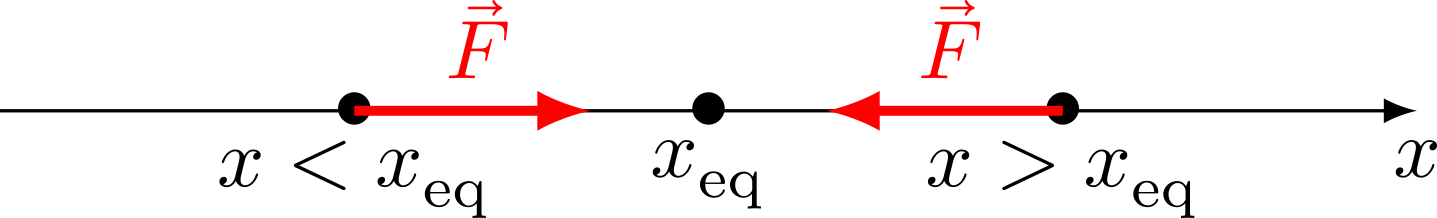
\includegraphics[width=\linewidth, draft=true]{stab_a-xeq}
			}{
				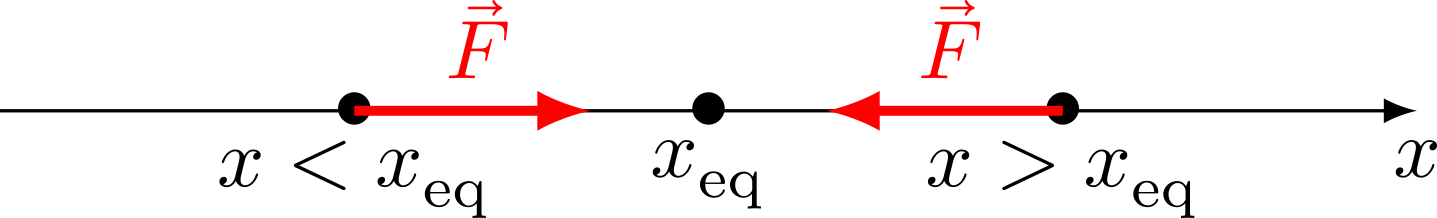
\includegraphics[width=\linewidth]{stab_a-xeq}
			}
			\vspace{-15pt}
			\captionof{figure}{Équilibre stable}
		\end{center}
	\end{minipage}
	\hfill
	\begin{minipage}{0.45\linewidth}
		\begin{center}
			\sswitch{
				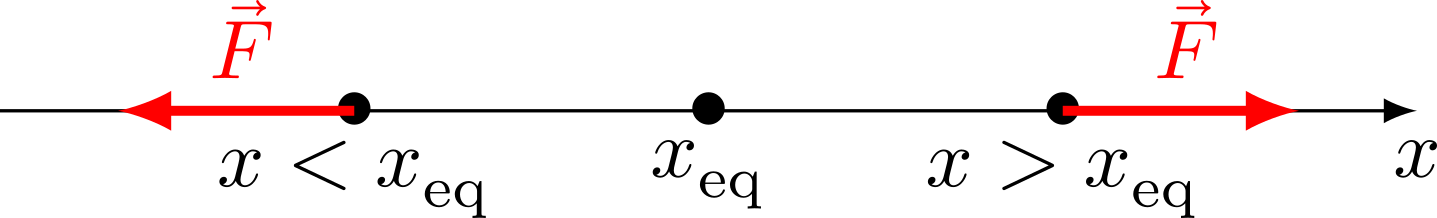
\includegraphics[width=\linewidth, draft=true]{instab_a-xeq}
			}{
				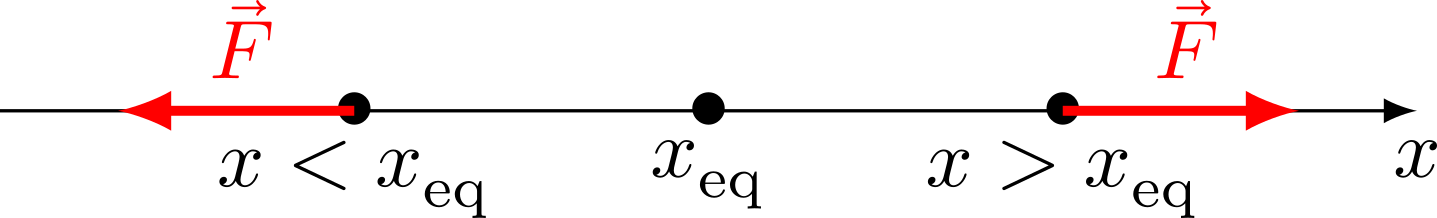
\includegraphics[width=\linewidth]{instab_a-xeq}
			}
			\vspace{-15pt}
			\captionof{figure}{Équilibre instable}
		\end{center}
	\end{minipage}
\end{tcb*}

Pour étudier ces situations mathématiquement, on peut développer l'expression de
la somme $\Ff$ au voisinage d'un point d'équilibre $x_{\equ}$ quelconque~:
\begin{DispWithArrows*}
	\psw{F(x)} &= \psw{F(x_{\equ}) + (x-x_{\equ})\times \eval{\dv{F}{x}}_{x_{\equ}}}
	\Arrow{$F = -\dv{\Ec_p}{x}$}
	\\\Lra
	\psw{F(x)} &=
	\psw{
	- \eval{\dv{\Ec_p}{x}}_{x_{\equ}} -
	(x-x_{\equ})\times\eval{\dv[2]{\Ec_p}{x}}_{x_{\equ}}
	}
	\Arrow{$F(x_{\equ}) = 0 = \eval{\dv{\Ec_p}{x}}_{x_{\equ}}$}
	\\\Lra
	\psw{F(x)} &= \psw{-(x-x_{\equ}) \eval{\dv[2]{\Ec_p}{x}}_{x_{\equ}}}
\end{DispWithArrows*}

\begin{itemize}
	\item Si c'est un équilibre \textbf{stable}, la force doit \textbf{ramener}
	      le point $x$ vers sa position d'équilibre~:
	      \psw{
		      \begin{gather*}
			      (x-x_{\equ}) > 0 \Ra F < 0
			      \Lra
			      \eval{\dv[2]{\Ec_p}{x}}_{x_{\equ}} > 0
		      \end{gather*}
	      }
	      et si $(x-x_{\equ}) < 0$, alors $F$ doit être $>0$, mais la conclusion
	      est la même.
	\item Si c'est un équilibre \textbf{instable}, la force doit
	      l'\textbf{écarter} de la position d'équilibre~:
	      \psw{
		      \begin{gather*}
			      (x-x_{\equ}) > 0 \Ra F > 0
			      \Lra
			      \eval{\dv[2]{\Ec_p}{x}}_{x_{\equ}} < 0
		      \end{gather*}
	      }
	      et si $(x-x_{\equ}) < 0$, alors $F$ doit être $<0$, mais la conclusion
	      est la même.
\end{itemize}

Le raisonnement se propage dans toutes les directions, on peut donc utiliser le
cas général à trois dimensions~:

\begin{tcb*}(prop){Stabilité des positions d'équilibre}
	Une position d'équilibre est~:\\
	\begin{isd}
		\[\text{\textbf{Stable} si}
			\qquad
			\psw{\boxed{\eval{\pdv[2]{\Ec_p}{x}}_{x_{\equ}} > 0}}
		\]
		\begin{center}
			\sswitch{
				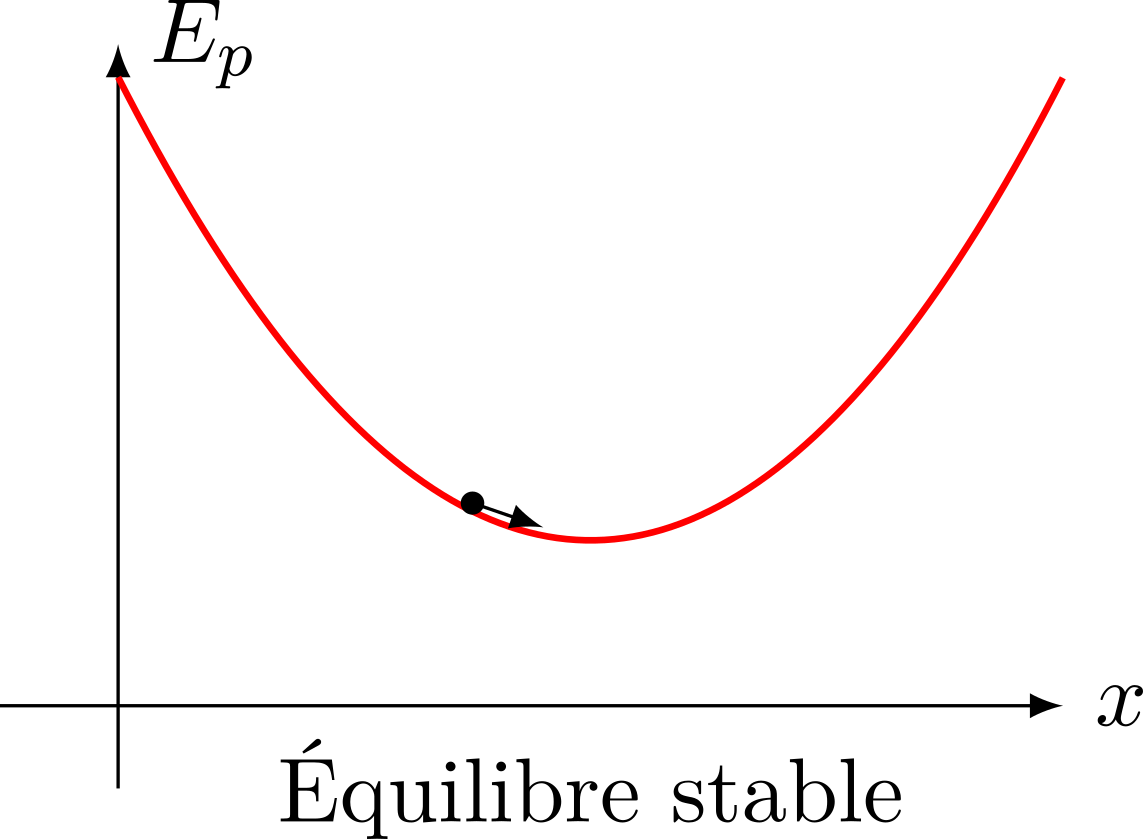
\includegraphics[width=6cm, draft=true]{stab_b}
			}{
				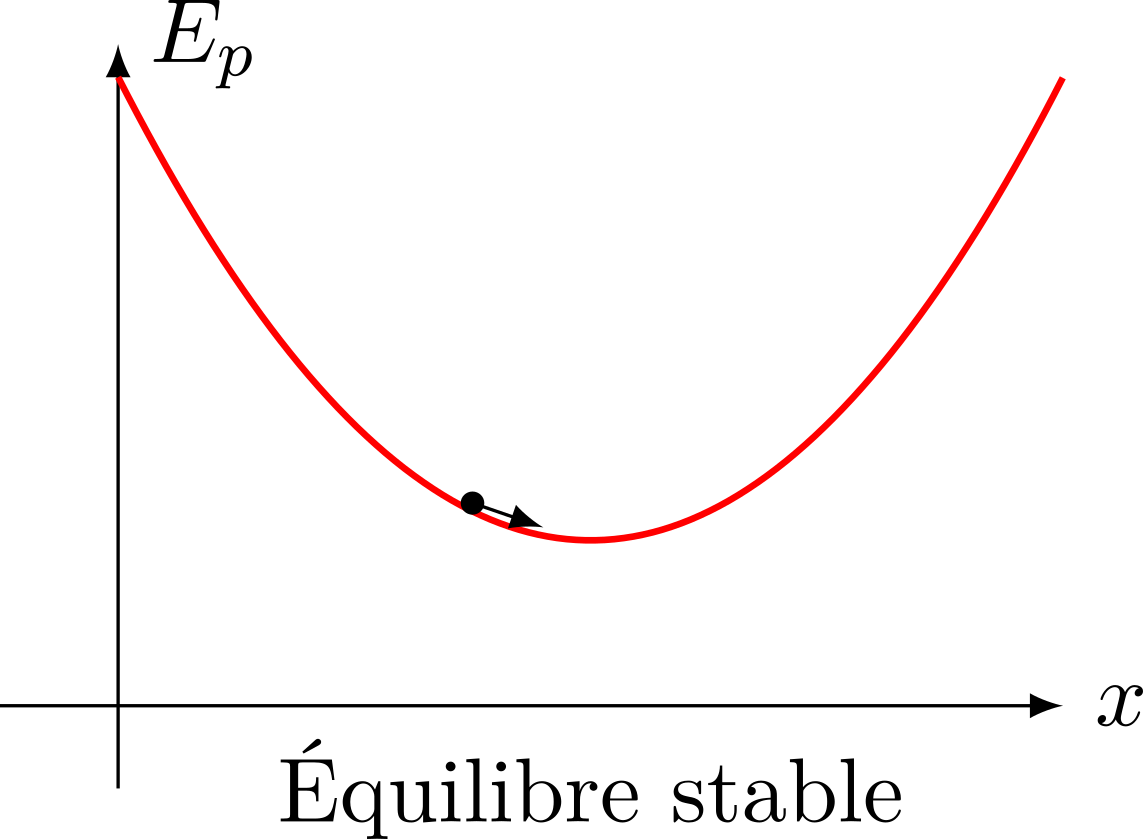
\includegraphics[width=6cm]{stab_b}
			}
			\vspace{-15pt}
			\captionof{figure}{Équilibre stable}
		\end{center}
		\tcblower
		\[\text{\textbf{Instable} si}
			\qquad
			\psw{\boxed{\eval{\pdv[2]{\Ec_p}{x}}_{x_{\equ}} < 0}}
		\]
		\begin{center}
			\sswitch{
				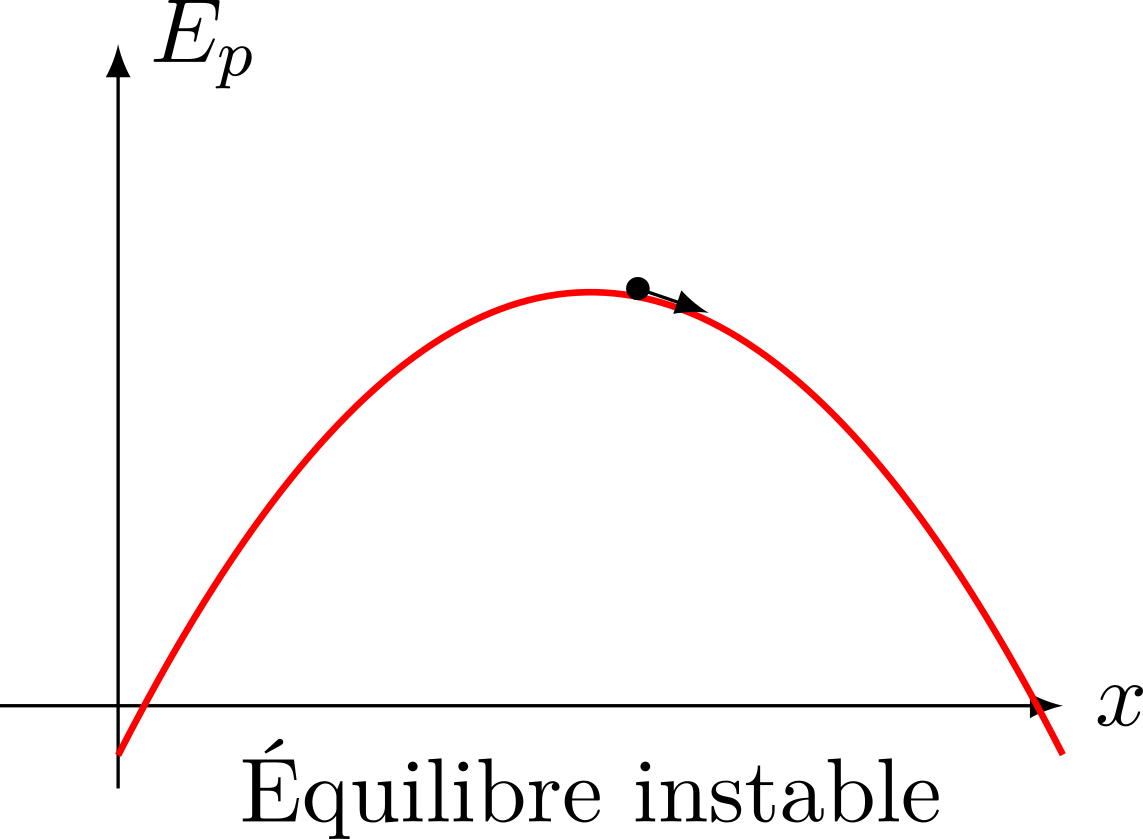
\includegraphics[width=6cm, draft=true]{instab_b}
			}{
				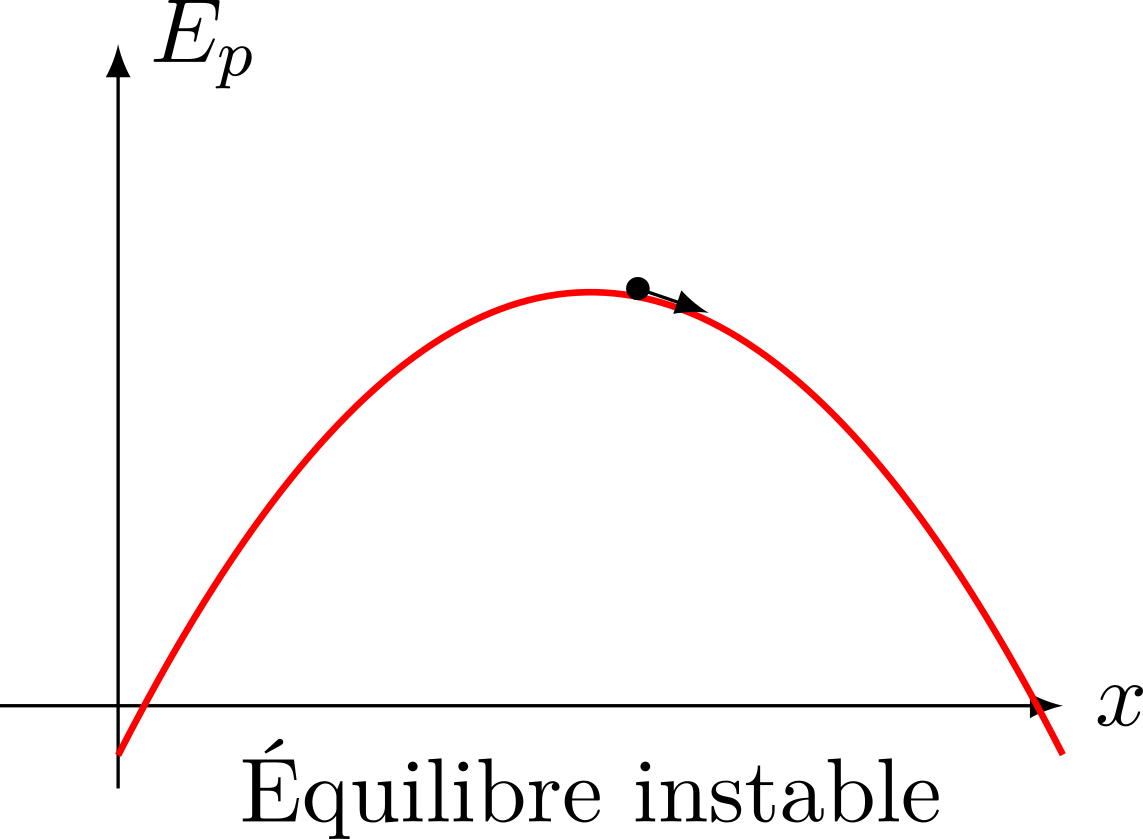
\includegraphics[width=6cm]{instab_b}
			}
			\vspace{-15pt}
			\captionof{figure}{Équilibre instable}
		\end{center}
	\end{isd}
\end{tcb*}

\begin{tcb*}(appl)<lftt>'l'{Équilibre d'un ressort par énergie potentielle}
	Trouver la position d'équilibre d'un ressort. Est-elle stable ou instable~?
	\tcblower
	\begin{minipage}{0.25\linewidth}
		\begin{center}
			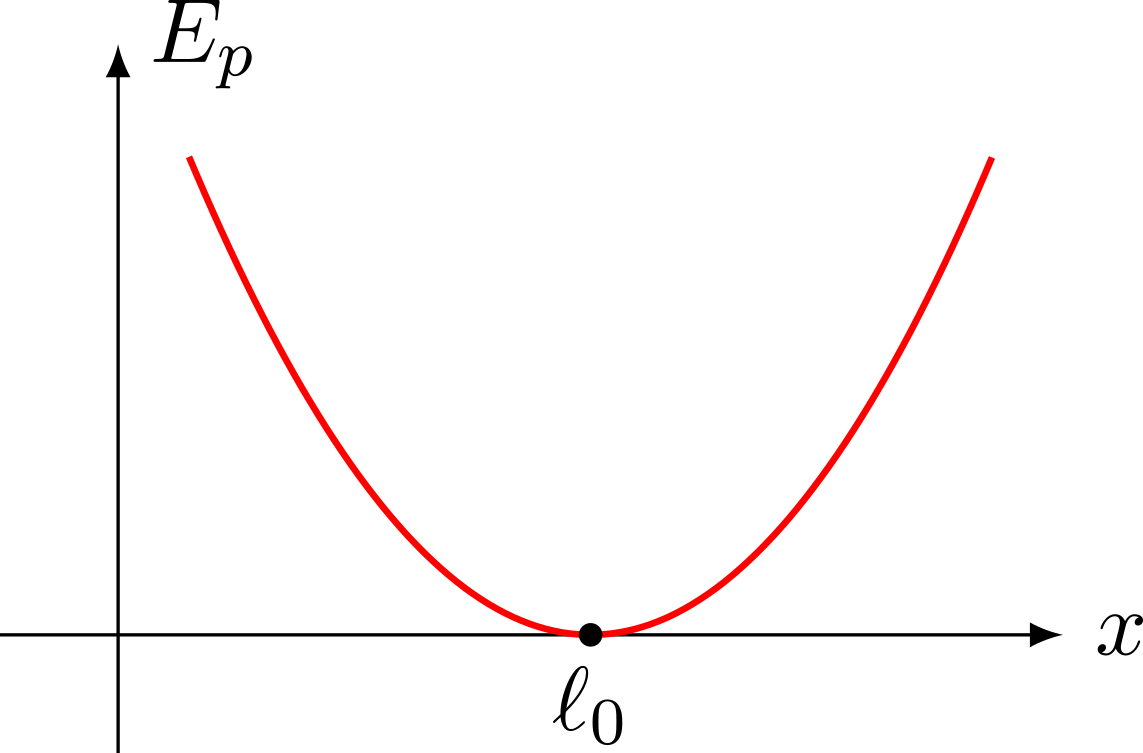
\includegraphics[width=\linewidth]{stab_ressort}
		\end{center}
	\end{minipage}
	\hfill
	\begin{minipage}{0.70\linewidth}
		\psw{
			L'énergie potentielle d'un ressort est
			\[
				\Ec_{p,\rm el} = \frac{1}{2}k(x-\ell_0)^2
				\Ra
				\dv{\Ec_{p,\rm el}}{x} = k(x-\ell_0)
				\Ra
				\dv[2]{\Ec_{p,\rm el}}{x} = k > 0
			\]
			Ainsi, la position d'équilibre est en $x_{\equ} = \ell_0$, et elle est
			stable.
		}
		\vspace{-15pt}
	\end{minipage}
\end{tcb*}

\subsection{Étude générale au voisinage d'un point d'équilibre stable}
En faisant un développement limité de l'énergie potentielle d'un système autour
d'une position d'équilibre stable, on a
\psw{
	\begin{gather*}
		\Ec_p(x) = \Ec_p(x_{\equ}) + (x-x\ind{eq})
		\underbracket[1pt]{\eval{\pdv{\Ec_p}{x}}_{x_{\equ}}}_{=0} +
		\frac{(x-x\ind{eq})^2}{2}
		\underbracket[1pt]{\eval{\pdv[2]{\Ec_p}{x}}_{x_{\equ}}}_{k}
		\\\Ra
		\Ec_m = \Ec_c + \Ec_p = \frac{1}{2}m\xp^2 + \frac{1}{2}k(x-x\ind{eq})^2
	\end{gather*}
}
\vspace{-15pt}
Et si l'énergie mécanique se conserve, on a $\DS\dv{\Ec_m}{t} = 0$ donc
\psw{
	\begin{gather*}
		\frac{1}{2}m(2\xpp\xp) + \frac{1}{2}k 2\xp(x-x_{\equ}) = 0
		\Lra
		\boxed{\xpp + \frac{k}{m}(x-x_{\equ}) = 0}
	\end{gather*}
}
On retrouve \psw{\textbf{l'équation de l'oscillateur harmonique}}~! Le mobile
oscille autour de la position d'équilibre à la pulsation $\w_0 = \sqrt{k/m}$
avec $k = \eval{\pdv[2]{\Ec_p}{x}}_{x_{\equ}}$.
\smallbreak
Ce qui est phénoménal, c'est que \textbf{la seule supposition est que le
	système soit conservatif}. Ceci explique l'abondance des systèmes harmoniques
dans la nature.

\begin{tcb*}(rema)<lftt>'l'{Étude mouvement équilibre instable}
	\begin{gather*}
		\beforetext{Si l'équilibre est instable~:}
		k = - \eval{\pdv[2]{\Ec_p}{x}}_{x_{\equ}} > 0
		\\
		\beforetext{d'où par le même raisonnement,}
		\xpp - \frac{k}{m}(x-x_{\equ}) = 0
		\\
		\beforetext{de solution}
		x-x_{\equ} = A\exr^{\w_0t} + B^{-\w_0t}
		\\
		\beforetext{Si $x(0) = x_0$ et $v(0) = 0$~:}
		x - x_{\equ} = x_0\cosh(\w_0t)
	\end{gather*}
	donc proche d'un point d'équilibre instable, le mobile \textbf{s'écarte
		exponentiellement} de cette position.
\end{tcb*}

\section{Énergie potentielle et trajectoire}

\subsection{Détermination qualitative d'une trajectoire}
Pour un point matériel soumis seulement à des forces conservatives (ou ne
travaillant pas), il est possible de prévoir les zones accessibles au mobile
ainsi que l'aspect de la trajectoire en étudiant l'énergie potentielle. En
effet,
\[\Ec_m = \Ec_c + \Ec_p \geq \Ec_p\]
puisque l'énergie cinétique est positive. Ainsi~:
\begin{tcb*}[breakable](ror){Trajectoire et énergie potentielle}
	Dans un diagramme d'énergie potentielle selon $x$~:
	\begin{itemize}
		\item \psw{Seules les régions où $\Ec_p \leq \Ec_m$ sont accessibles~;}
		\item \psw{
			      Lorsque $\Ec_p = \Ec_m$, $\Ec_c = 0$ donc la vitesse est nulle~;
		      }
		\item \psw{
			      Lorsque $\Ec_p$ est minimale, $\Ec_c$ est maximale donc la vitesse
			      est maximale.
		      }
		      % \item Si les valeurs de $x$ sont \textbf{bornées}, on dit que le système
		      %     est dans un \textbf{état lié}~;
		      % \item Si les valeurs de $x$ peuvent tendre vers \textbf{l'infini}, le
		      %     système est dans un \textbf{état de diffusion}
	\end{itemize}\bigbreak
	\begin{isd}
		\tcbsubtitle{\fatbox{État lié}}
		La particule reste dans une zone bornée de l'espace et le mobile effectue
		des aller-retours périodiques autour de la position d'équilibre.
		\begin{center}
			\sswitch{
				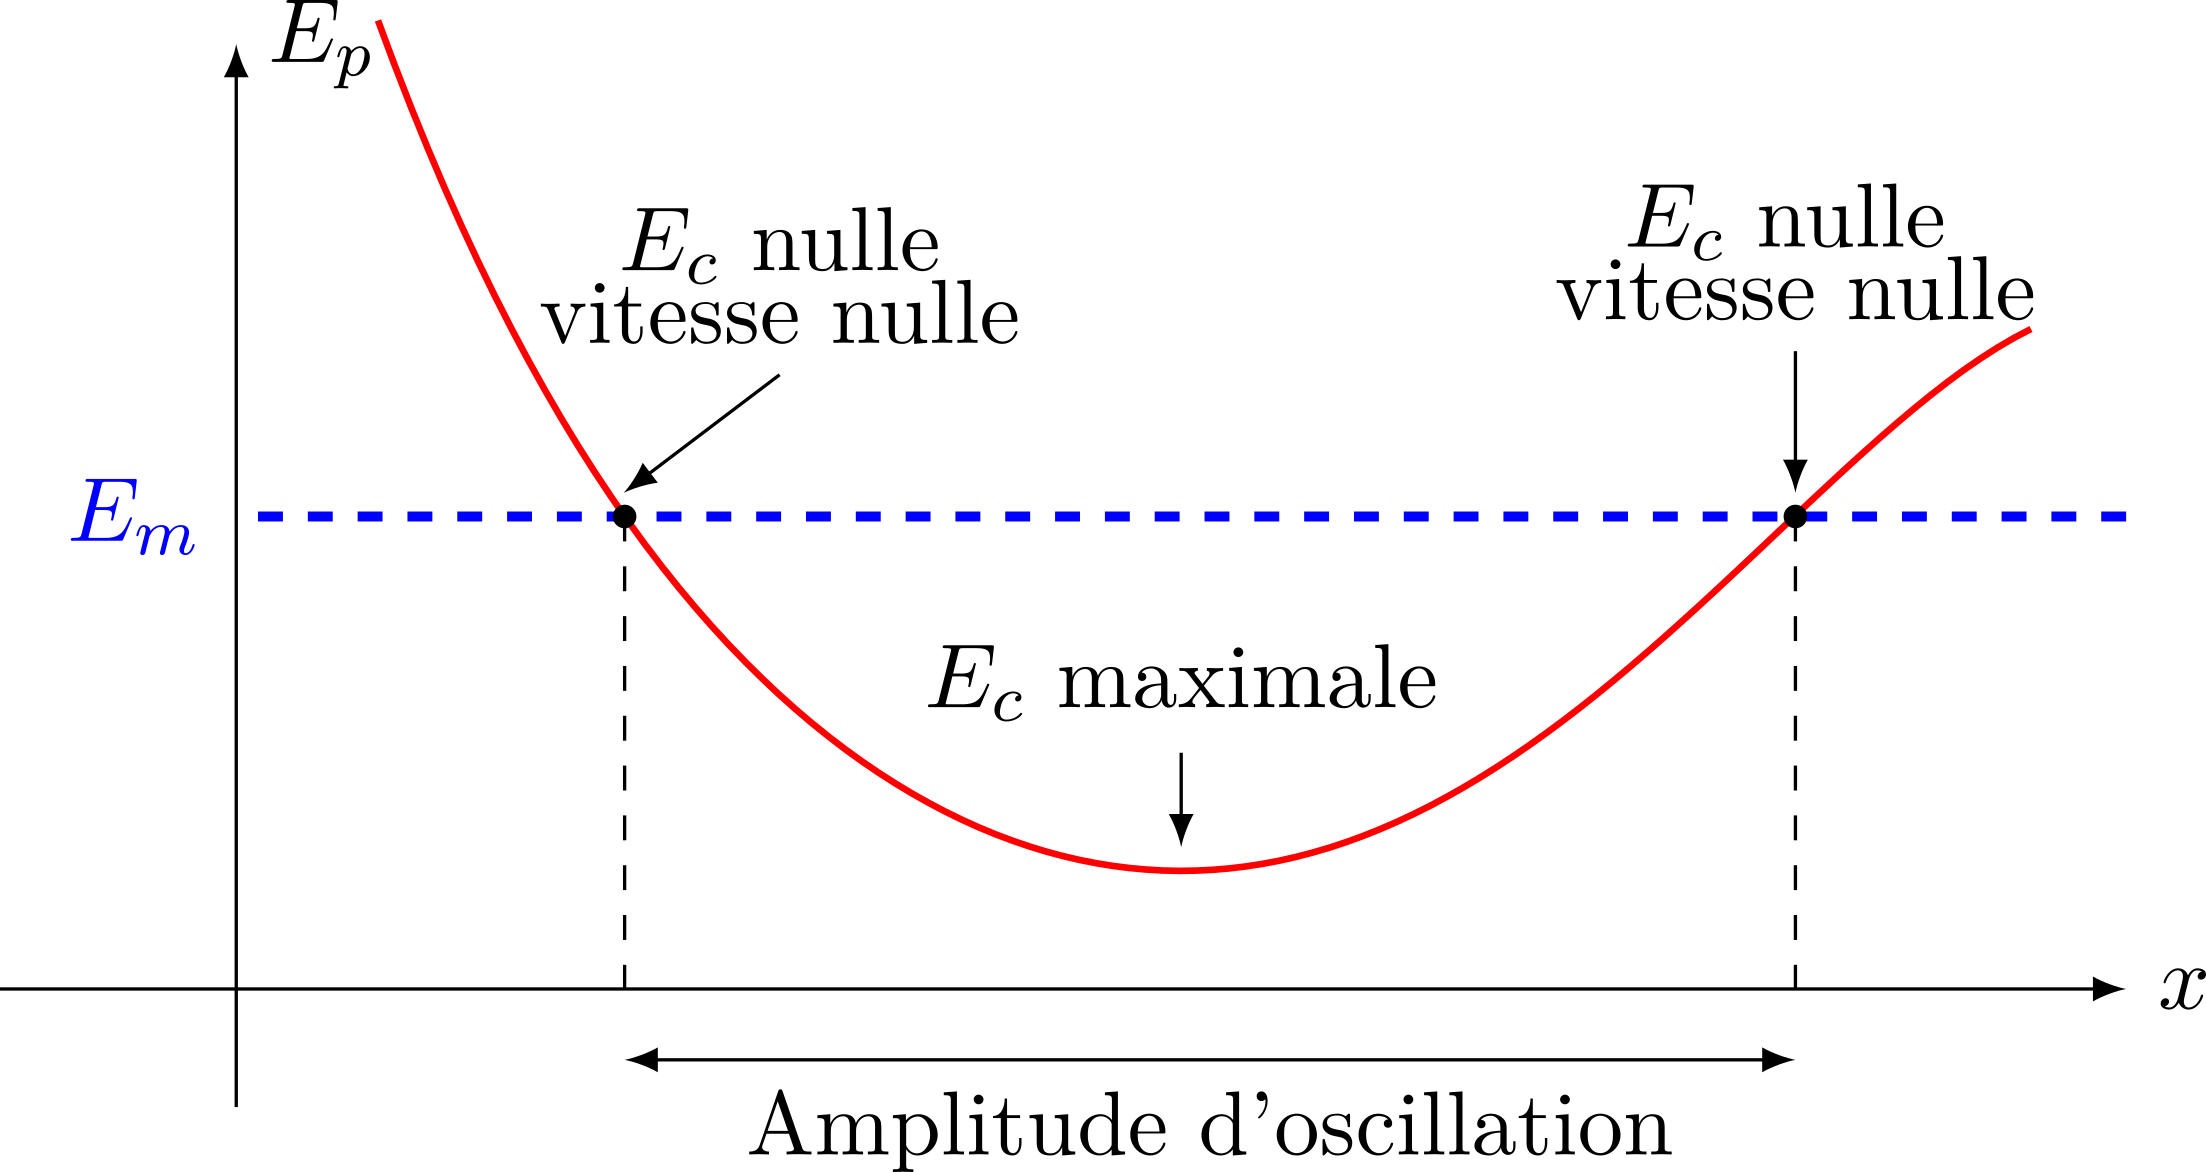
\includegraphics[width=7cm, draft=true]{stab_lie}
			}{
				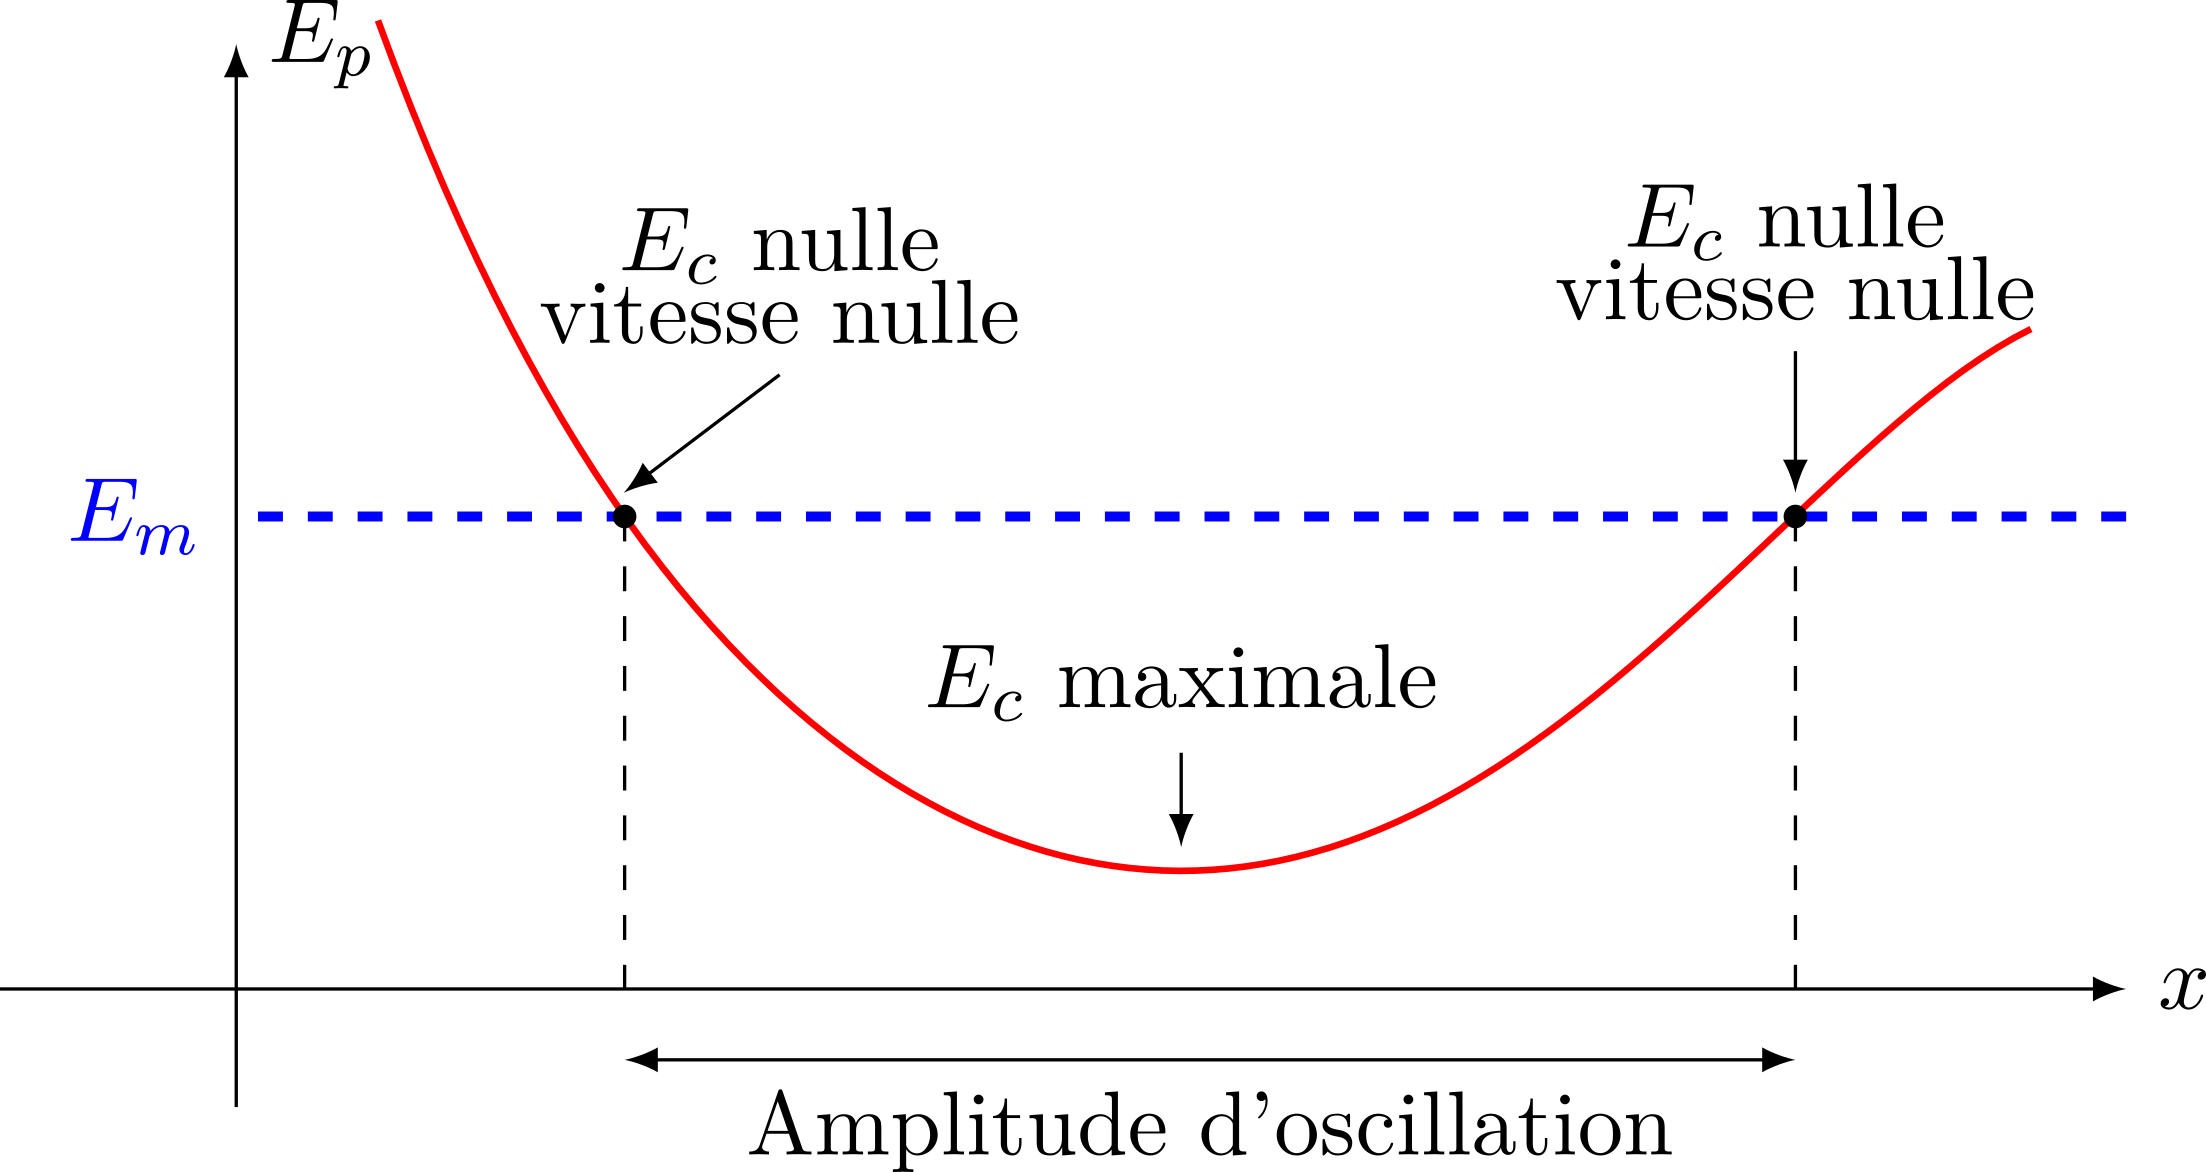
\includegraphics[width=7cm]{stab_lie}
			}
			\captionof{figure}{État lié}
		\end{center}
		\tcblower
		\tcbsubtitle{\fatbox{État de diffusion}}
		La particule aura tendance à partir vers $x = +\infty$ sans jamais revenir~:
		son mouvement n'est pas borné dans l'espace.
		\begin{center}
			\sswitch{
				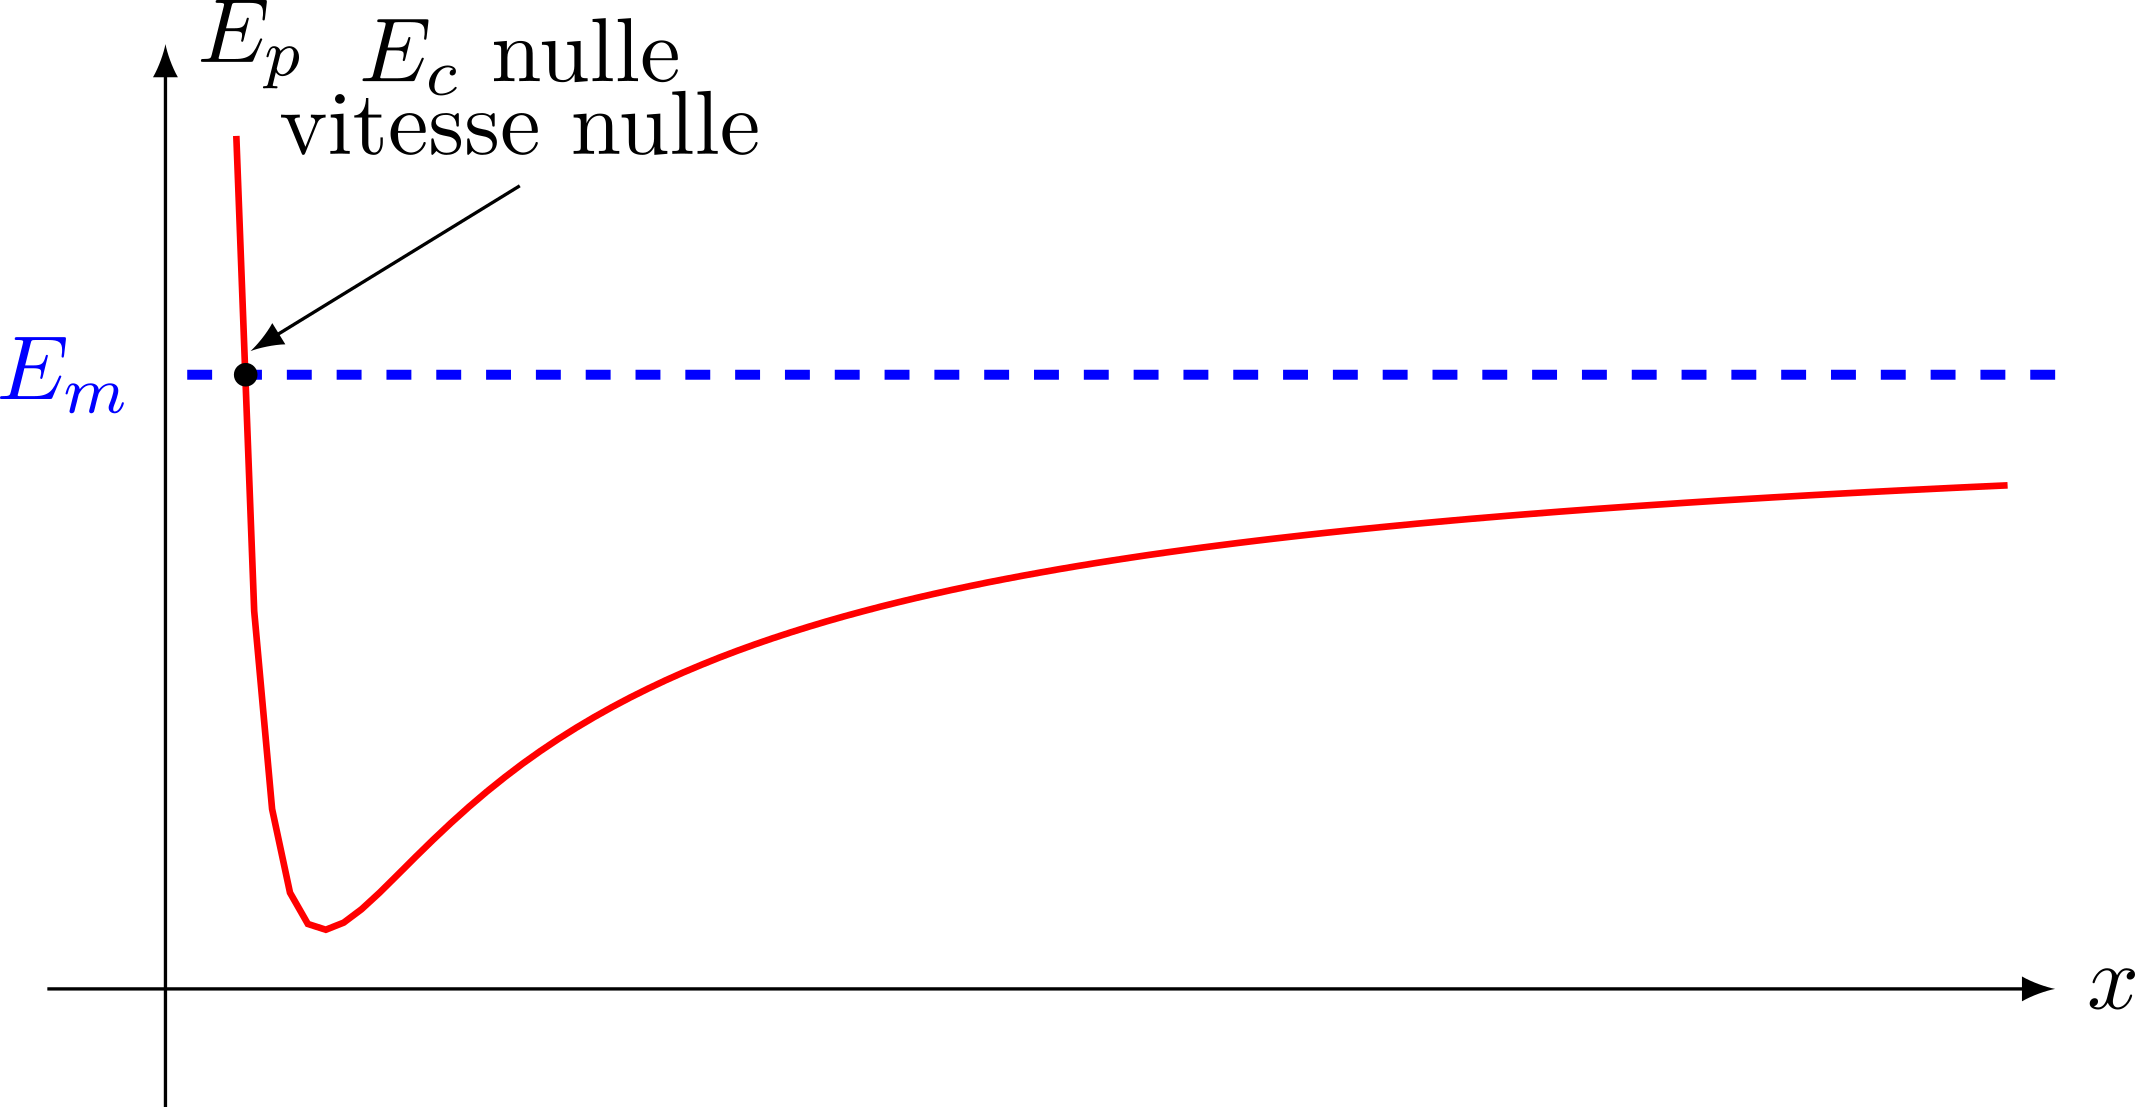
\includegraphics[width=7cm, draft=true]{stab_diff}
			}{
				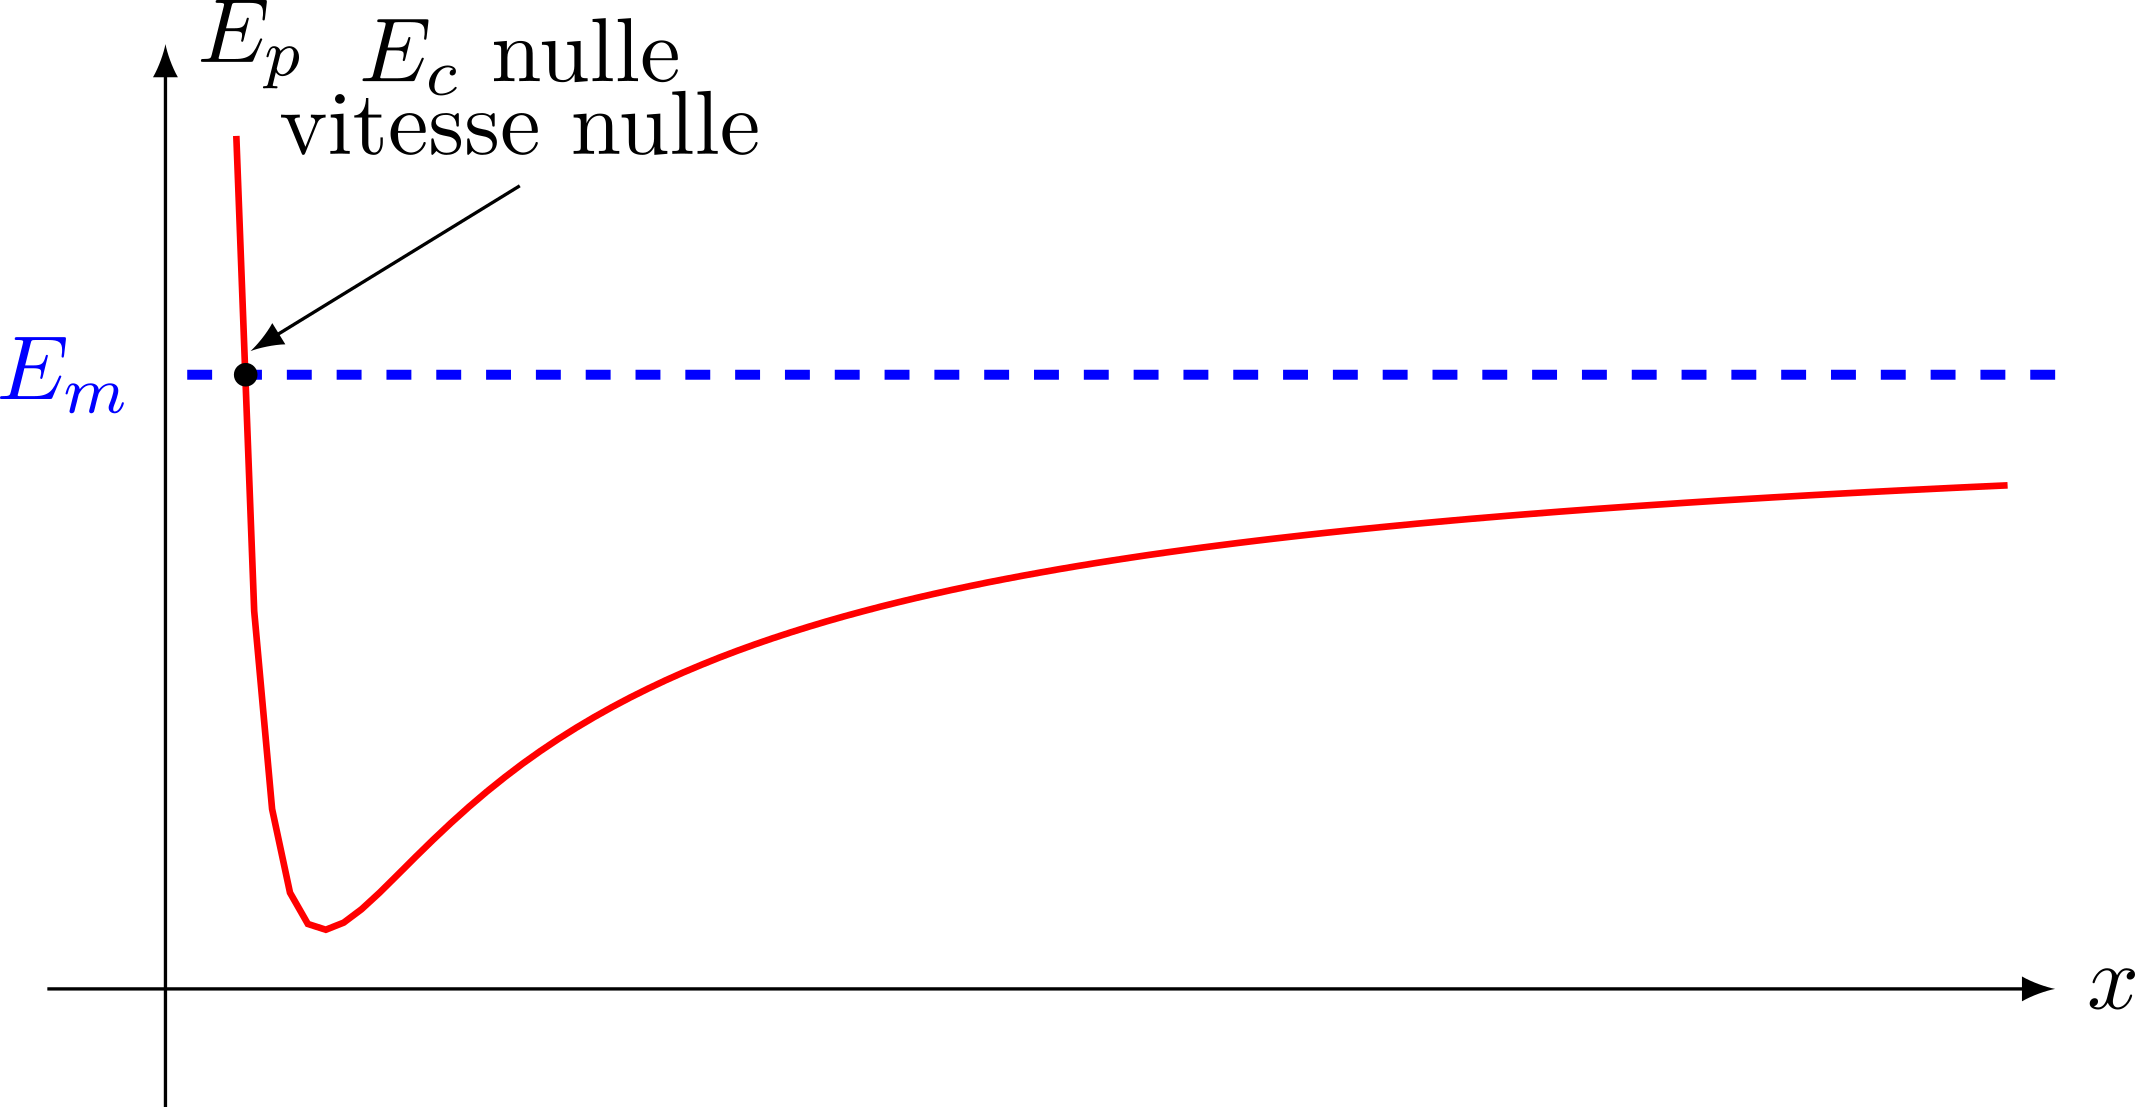
\includegraphics[width=7cm]{stab_diff}
			}
			\captionof{figure}{État de diffusion}
		\end{center}
	\end{isd}
\end{tcb*}

Certains corps célestes sont dans des états liés, comme la Terre et le Soleil,
d'autres dans des états de diffusion~: ils passent brièvement dans le système
solaire avant de le quitter définitivement. C'est le cas de la comète
d'\textsc{Arend-Roland}, passée à proximité de la Terre en 1956 mais qui ne
devrait jamais revenir.

\subsection{Cas du pendule simple}
On reprend le pendule simple, que l'on suppose attaché avec une tige
\textbf{rigide} (pour éviter les décrochages). On souhaiterait déterminer ses
positions d'équilibre et étudier ses trajectoires possibles. Le système étant
conservatif ($\Pf$ conservatif et $\Tf\perp\vf$), déterminons l'expression de
l'énergie potentielle en fonction de l'angle.
\begin{gather*}
	\beforetext{L'altitude est~:}
	\psw{z(\tt) = \ell(1-\cos\tt)}
	\\
	\beforetext{donc l'énergie potentielle est}
	\psw{\boxed{\Ec_p(\tt) = mgz(\tt) = mg\ell(1-\cos\tt)}}
\end{gather*}

\begin{center}
	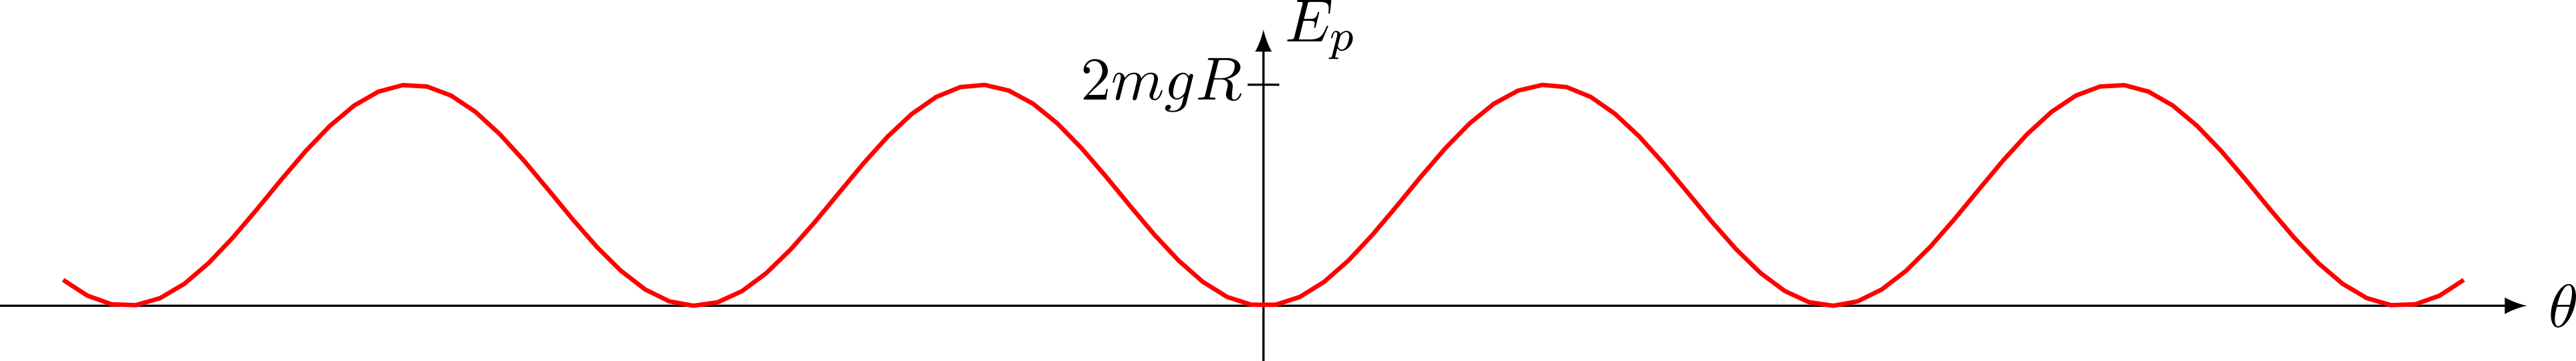
\includegraphics[scale=1]{stab_pend-a}
\end{center}
Les positions d'équilibre stables sont donc celles dans les «~creux~», soit $\tt =
	2p\pi$ avec $p\in\Zb$, et les instables sur les «~collines~», soit $\tt =
	(2p+1)\pi$. On distingue alors deux cas~:

\subsubsection{Cas $\Ec_m < 2mg\ell$}
Si l'énergie mécanique totale est inférieure à l'énergie potentielle maximale, on se
situera dans un état lié, «~coincé~» dans un creux. On observera donc une
oscillation autour du point d'équilibre le plus proche, et on a vu que cette
oscillation état sinusoïdale aux très petits angles ($\abs{\tt} < \ang{20}$).

\begin{minipage}{0.45\linewidth}
	\begin{center}
		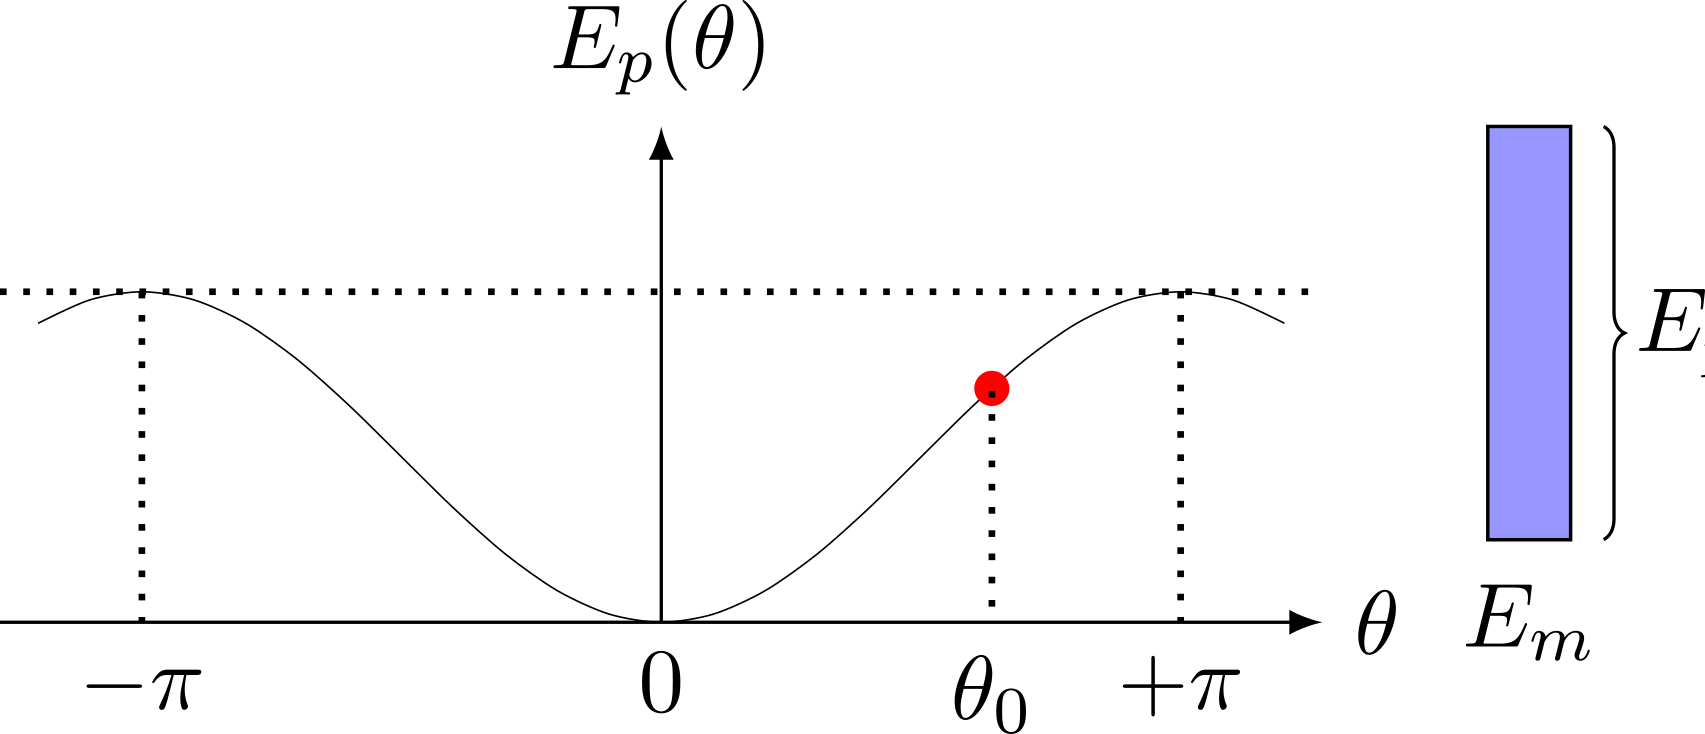
\includegraphics[width=7cm]{stab_pend-b}
		\captionof{figure}{État initial $\tt = \tt_0$~: toute l'énergie est sous
			forme d'énergie potentielle, et l'énergie est nulle.}
	\end{center}
\end{minipage}
\hfill
\begin{minipage}{0.45\linewidth}
	\begin{center}
		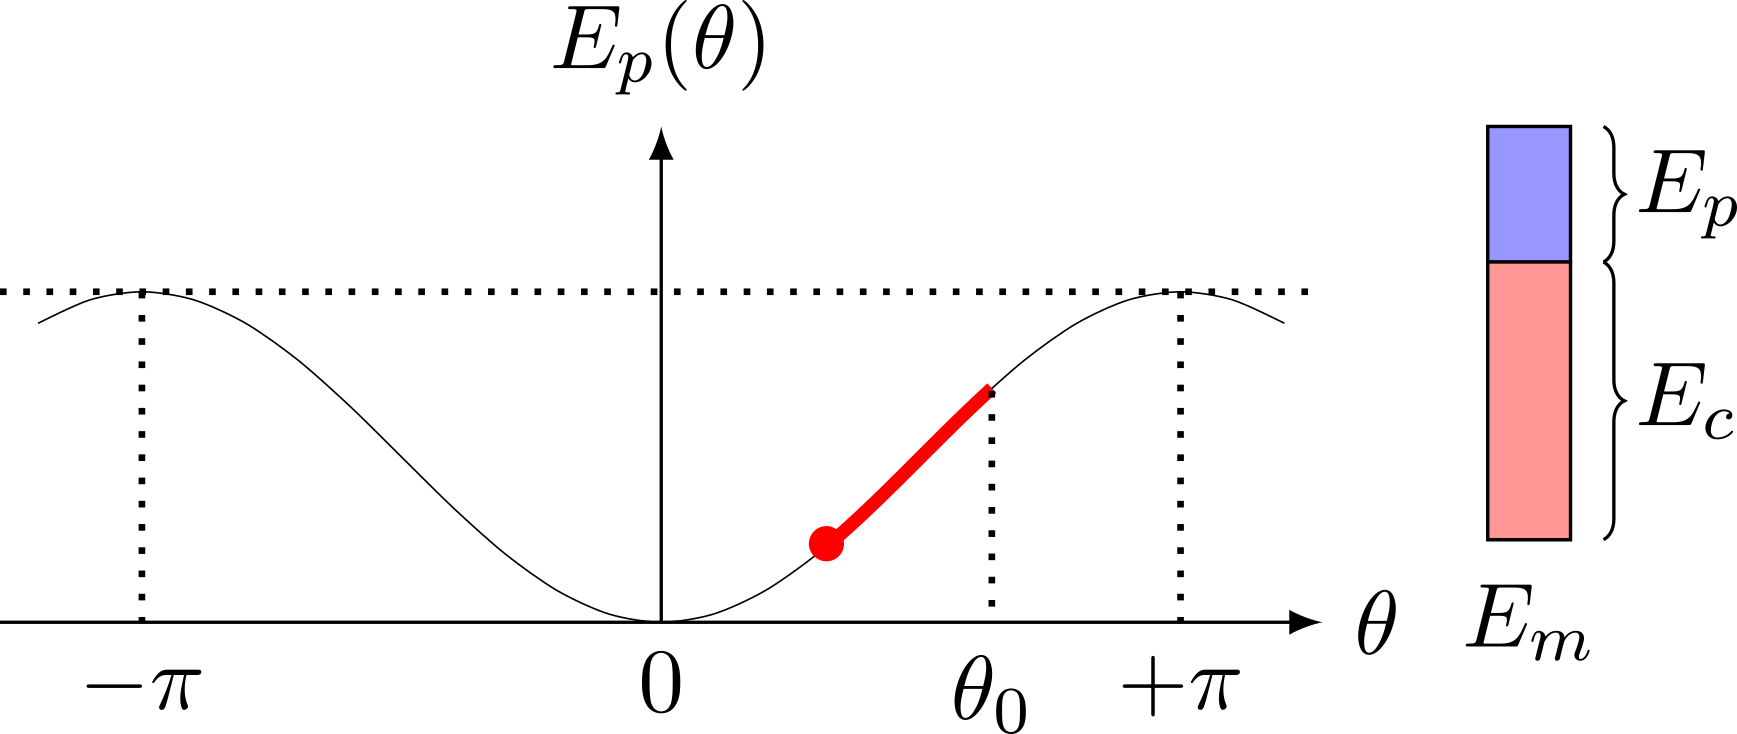
\includegraphics[width=7cm]{stab_pend-c}
		\captionof{figure}{La masse perd de l'énergie potentielle tout en restant sur
			la courbe. L'énergie mécanique étant conservée, elle gagne de l'énergie
			cinétique et donc de la vitesse.}
	\end{center}
\end{minipage}

\begin{minipage}{0.45\linewidth}
	\begin{center}
		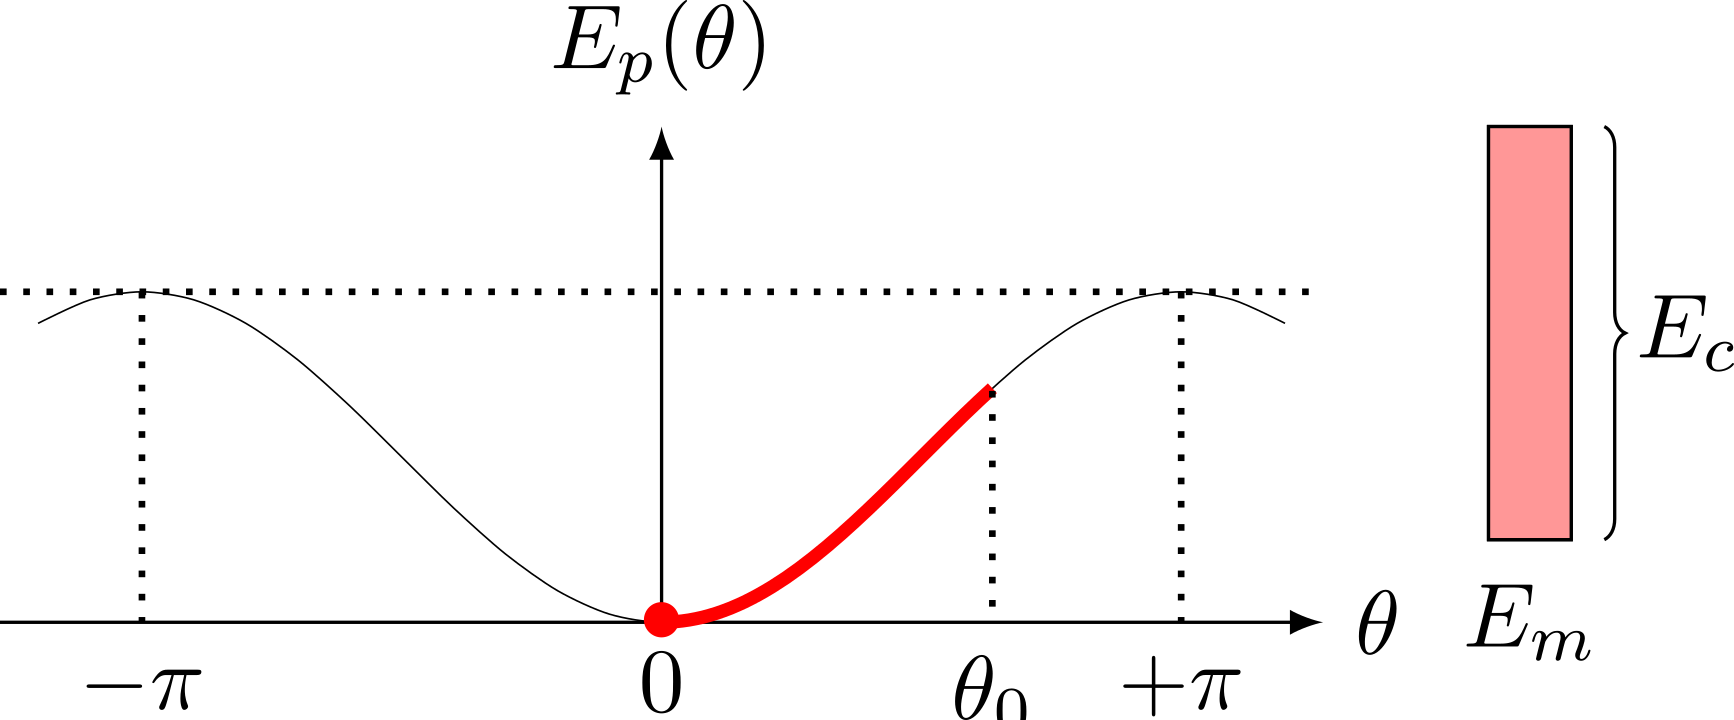
\includegraphics[width=7cm]{stab_pend-d}
		\captionof{figure}{La masse a perdu toute son énergie potentielle~: son
			énergie cinétique et donc sa vitesse sont maximales.}
	\end{center}
\end{minipage}
\hfill
\begin{minipage}{0.45\linewidth}
	\begin{center}
		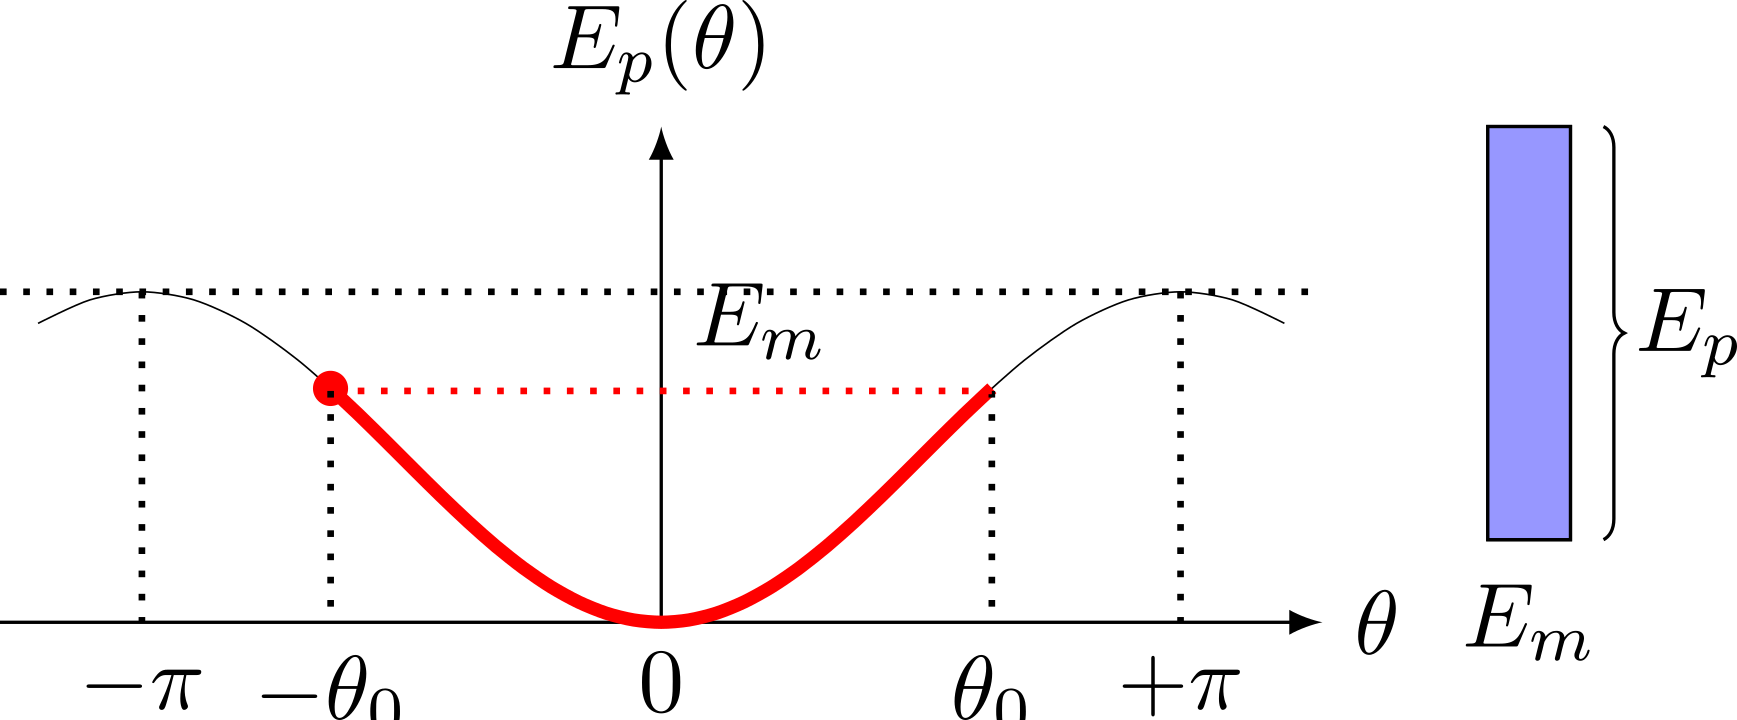
\includegraphics[width=7cm]{stab_pend-e}
		\captionof{figure}{La masse a perdu toute son énergie cinétique et a
			maximisé son énergie potentielle. Elle a atteint l'angle maximale
			$-\tt_0$, et repart dans l'autre sens.}
	\end{center}
\end{minipage}

\vspace{-15pt}
\subsubsection{Cas $\Ec_m > 2mg\ell$}
Si l'énergie mécanique totale est supérieure à l'énergie potentielle maximale,
ça veut dire qu'il y a un excédent d'énergie cinétique. Ainsi, le pendule tourne
autour de l'axe de rotation, et lorsqu'il arrive en $\tt = \pi$ l'énergie
potentielle est maximale mais l'énergie cinétique n'est pas nulle~: il continue
sa rotation, sans oscillation. La vitesse n'est cependant pas constante, elle
est plus faible en haut qu'en bas du mouvement (par conservation de l'énergie
mécanique).

Une animation est disponible en
ligne\footnote{\url{https://phyanim.sciences.univ-nantes.fr/Meca/Oscillateurs/tension_pendule.php}}.

\end{document}
